\documentclass[AER]{AEA}
\usepackage{natbib}
\usepackage{amsmath,amssymb}
\usepackage{booktabs}
\usepackage{graphicx}
\usepackage{multirow}
\draftSpacing{1.5}

\begin{document}

\title{Abundant Capital, Scarce Appropriability: Development Finance during the AI Investment Boom}
\shortTitle{Development Finance during the AI Boom}
\author{Werner Hernani-Limarino\thanks{Hernani-Limarino: AI Analytics and Bolivian Academy of Economic Sciences (wernerhl@gmail.com). This paper is the descriptive companion to ``AI Capital and the Crowding Out of Development Investment.'' All data are public and the construction code is available in the replication repository.}}
\date{\today}
\pubMonth{Month}
\pubYear{Year}
\pubVolume{Vol}
\pubIssue{Issue}
\JEL{F21, F34, F35, O19, O33}
\Keywords{artificial intelligence, capital expenditure, official development assistance, international bond markets, low-income countries}

\begin{abstract}
This paper assembles the public record on how the artificial-intelligence investment boom has been financed and what happened to development finance over the same period. Capital expenditure by the five largest cloud providers rose from USD 154 billion in 2023 to a USD 691 billion annual rate in 2026 and, since late 2025, is funded by bond issuance of USD 45--80 billion per quarter rather than cash flow. Official development assistance fell 23 percent in real terms in 2025, concentrated in the United States and in grants for health, humanitarian relief and government services. Yet the bond market shows no scarcity of capital: international financial institutions raised 44 percent more, emerging-market sovereigns 27 percent more, and announcement-day tests find no effect of AI return shocks on the cost of capital of developing countries. What contracted is financing whose returns cannot be appropriated by the funder. Thirty-two countries with 400 million people, mostly in Sub-Saharan Africa, depend on such financing for more than 5 percent of national income and have no access to markets; the 2025 cut lands on them through HIV programmes and humanitarian relief.
\end{abstract}

\maketitle

The question that motivates this paper is whether the investment boom in artificial intelligence has drawn capital away from the investments on which the poorest part of the world population depends. The companion theoretical paper formalizes one channel through which this could happen: AI capital and development capital are financed from a common pool, funders appropriate only part of the return to development capital, and an increase in the return to AI raises the hurdle rate on all investment. This paper does something more modest and prior. It assembles, from public sources only, the facts that any explanation of the coincidence between the AI boom and the collapse of development assistance must accommodate, and it reports them without imposing the model.

Two facts are not in dispute. Capital expenditure by the five largest cloud providers rose from USD 154 billion in calendar 2023 to a USD 691 billion annual rate by the third quarter of 2026, and official development assistance (ODA) from the members of the OECD Development Assistance Committee (DAC) fell by 23 percent in real terms in 2025, the largest decline on record \citep{OECD2026ODA}. The purpose of the exercise is to establish what lies between these two facts: how the capital expenditure is financed, who else raises money on the same markets, whether the cost of capital faced by developing countries responds to AI news, which donors cut, which recipients and sectors lost, and which countries have no alternative source of finance.

The findings do not support the simplest version of the crowding-out story, in which a scarce pool of loanable funds is bid away by AI. Capital is abundant. The stock of international bonds outstanding grew 42 percent between the end of 2019 and mid-2026; development banks doubled their borrowing; emerging-market governments issued more, not less; cross-border bank lending to developing economies rose fivefold. The hyperscalers began drawing on external finance only in the last quarter of 2025, so the period in which they could have competed with anyone for funds is a year old. On announcement days, news about AI returns does not raise the spreads of developing-country borrowers once common risk factors are controlled for, and the one shock that does, surprises in realized capital expenditure, raises US high-yield spreads by as much.

What the facts do support is a narrower and, I will argue, sharper reading. The financial system allocates abundant capital to whatever has returns that funders can collect: AAA paper issued by development banks, cloud capacity with contracted revenue, sovereign Eurobonds of middle-income countries, and, within development finance, the ``mobilised'' private flows that go overwhelmingly to financial intermediaries and energy. The financing that contracted is the financing of services with no collectable return at all: grant aid for health, humanitarian relief and the functioning of governments in countries that cannot borrow. The scarce factor is not capital but appropriability. Section~\ref{sec:interp} states what this implies for the three explanations of the 2025 collapse that the companion paper sets out, and for the model itself.

\section{Data}\label{sec:data}

All series are public and are reconstructed by the code in the replication repository. Firm-level data come from SEC EDGAR: quarterly capital expenditure, cash from operations, long-term debt issued and repaid, share repurchases and dividends for Microsoft, Alphabet, Amazon, Meta and Oracle (the hyperscalers) and for Nvidia, Broadcom and AMD, de-cumulated from the year-to-date figures that 10-Q filings report, together with the filing dates of 8-K earnings releases. Daily prices for these firms, for a basket of AI suppliers (TSMC, Vertiv, Arista, Super Micro, Micron, ASML), for the S\&P 500 and for emerging-market bond and equity exchange-traded funds come from Yahoo Finance, as do announcement timestamps and consensus earnings surprises. Treasury yields, the VIX, the broad dollar index, and ICE BofA option-adjusted spreads for emerging-market and US corporate indices come from FRED; the Fama--French factors from Kenneth French's library \citep{Fama1993}.

Development finance comes from the OECD \citep{OECD2026CRS}: ODA by donor including the preliminary 2025 figures (DAC1), ODA received by recipient country, region and income group from all official donors and from the United States (DAC2A), bilateral commitments by sector and donor (DAC5), disbursements by recipient and purpose sector from the Creditor Reporting System (CRS), and private finance mobilised by official interventions by recipient, sector and instrument. Country-level external flows (ODA received, foreign direct investment, portfolio equity, remittances, capital formation) and external-debt flows by creditor type come from the World Bank's World Development Indicators and International Debt Statistics \citep{WB2026IDS}. Cross-border bank claims on developing economies, quarterly and adjusted for exchange rates and breaks, and international debt securities issuance by residence and sector of issuer, including the international organisations category that captures the multilateral development banks and other supranationals, come from the Bank for International Settlements \citep{BIS2026IDS}. US investment by type comes from the Bureau of Economic Analysis and the Federal Reserve's financial accounts, and construction spending by category, including data centers, from the Census Bureau.

Three constructed series are used in Section~\ref{sec:prices}. The first is the two-day abnormal return of each AI firm around each of its 133 earnings releases between October 2022 and November 2026, from a Fama--French five-factor model with momentum estimated over the preceding year. The second is a capital-expenditure surprise, realized quarterly capex minus a seasonal random walk with drift, scaled by lagged assets, which substitutes for the consensus capex forecasts that are not freely available. The third is a daily AI factor, the equal-weighted return of the AI basket net of the market and the Fama--French factors. Throughout, ``pre'' denotes the period 2019 to the third quarter of 2022 and ``post'' the period from the first quarter of 2023, the release of ChatGPT on 30 November 2022 being the conventional start of the boom.

\section{The AI investment boom and its financing}\label{sec:boom}

Table~\ref{tab:hyp} reports the annual accounts of the five hyperscalers. Capital expenditure doubled between 2019 and 2022, was flat in 2023, and then rose by 55 percent in 2024, 72 percent in 2025 and, on the first three quarters, around 80 percent in 2026. Through 2024 the expansion was financed entirely from operations: cash from operations exceeded capex by a factor of two, net debt issuance was negligible, and the firms returned more to shareholders through repurchases than they invested. The financing changed in the fourth quarter of 2025. Capex overtook cash from operations in the first quarter of 2026, long-term debt issuance rose to USD 45, 80 and 48 billion in the three quarters from 2025Q4 to 2026Q2, and share repurchases fell from about USD 30 billion a quarter to under USD 5 billion. The year-to-date 2026 debt issuance of USD 143 billion is larger than the sum of the previous seven years. These figures exclude lease obligations and the joint ventures with private-credit funds through which a growing share of data-center capacity is financed off balance sheet, so they understate the claim of AI on external capital.

\begin{table}
\caption{Hyperscaler capital expenditure and its financing, USD billion}\label{tab:hyp}
\resizebox{\textwidth}{!}{\begin{tabular}{lrrrrrrrr}
\toprule
 & 2019 & 2020 & 2021 & 2022 & 2023 & 2024 & 2025 & 2026 (Q1--Q3) \\
\midrule
Capital expenditure & 71 & 97 & 131 & 158 & 154 & 239 & 412 & 560 \\
Cash from operations & 197 & 252 & 290 & 288 & 377 & 478 & 603 & 543 \\
Long-term debt issued & 1 & 11 & 19 & 59 & 5 & 16 & 53 & 143 \\
Share repurchases & 68 & 82 & 151 & 124 & 102 & 111 & 95 & 14 \\
Dividends & 17 & 19 & 21 & 22 & 25 & 40 & 46 & 31 \\
\bottomrule
\end{tabular}}
\begin{tablenotes}
Sum over Microsoft, Alphabet, Amazon, Meta and Oracle, from 10-Q and 10-K cash-flow statements (SEC EDGAR), de-cumulated to quarters and summed by calendar year of period end. Debt issued is gross proceeds from long-term debt.
\end{tablenotes}
\end{table}


\begin{figure}
\centering
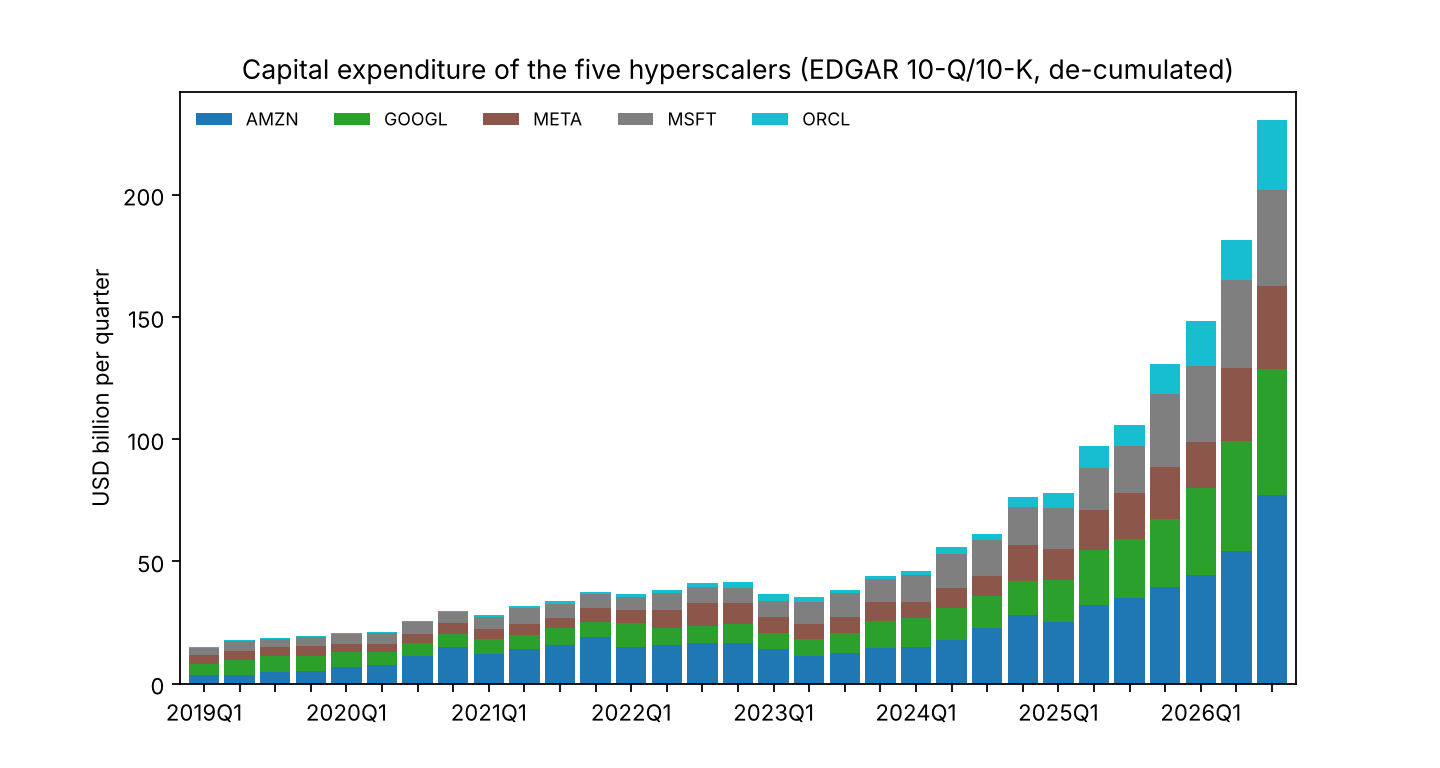
\includegraphics[width=\textwidth]{figures/fig_capex.png}
\caption{Quarterly capital expenditure of the five hyperscalers}\label{fig:capex}
\begin{figurenotes}
Quarterly capex by firm from 10-Q and 10-K cash-flow statements (SEC EDGAR), de-cumulated from year-to-date figures. Dashed line: release of ChatGPT, November 2022.
\end{figurenotes}
\end{figure}

\begin{figure}
\centering
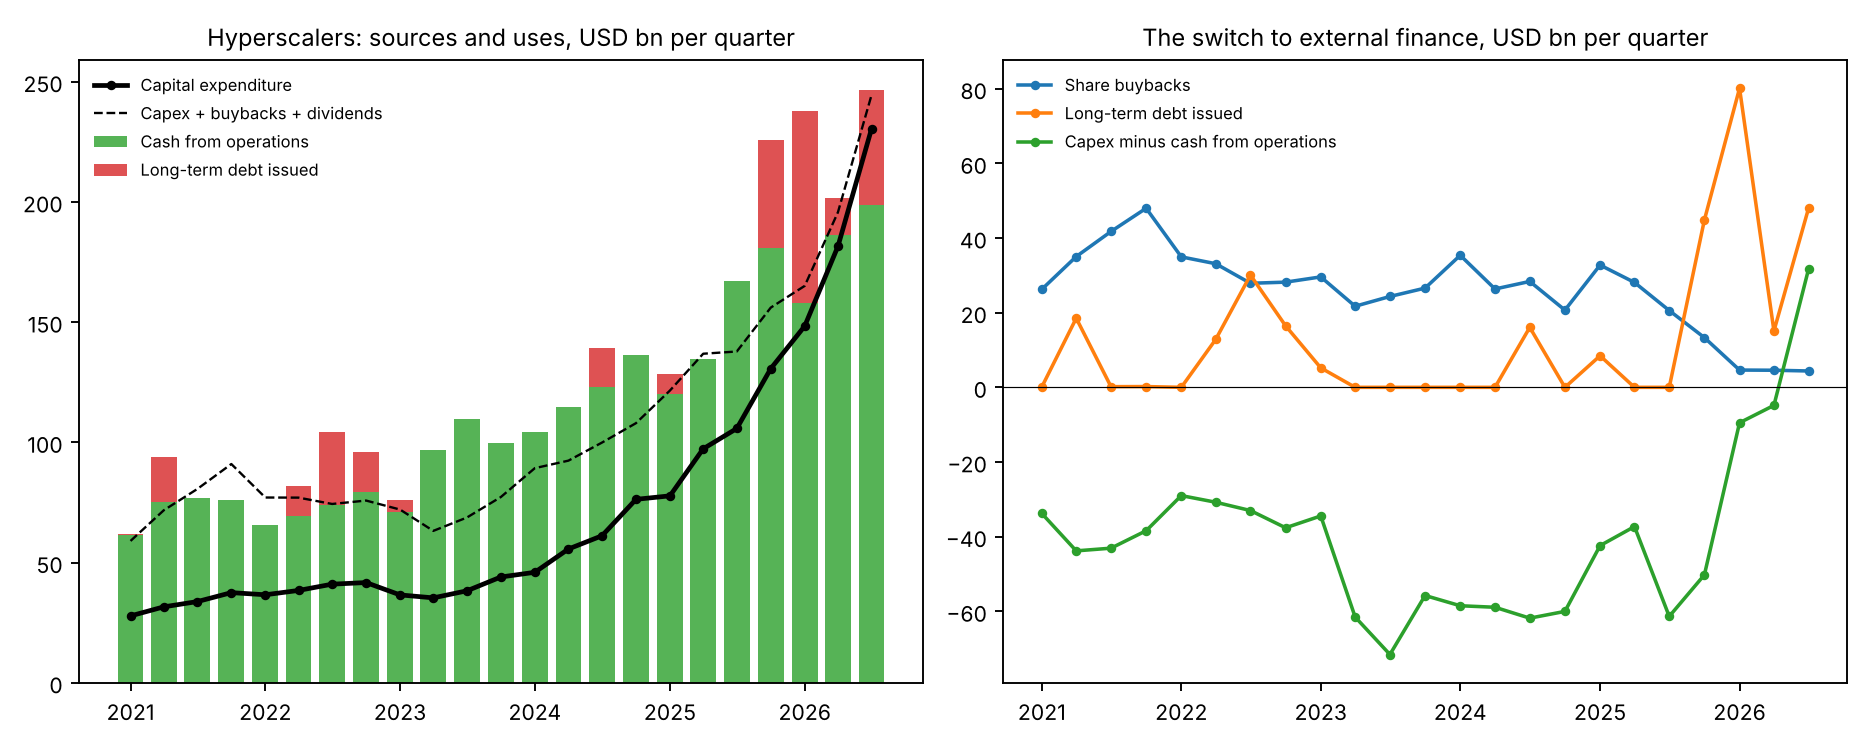
\includegraphics[width=\textwidth]{figures/fig_hyperscaler_funding.png}
\caption{How the hyperscalers fund capital expenditure}\label{fig:funding}
\begin{figurenotes}
Left: cash from operations and long-term debt issued (stacked bars) against capital expenditure and capital expenditure plus buybacks and dividends (lines), USD billion per quarter, sum over the five firms. Right: share repurchases, long-term debt issued, and capex minus cash from operations.
\end{figurenotes}
\end{figure}
Figure~\ref{fig:capex} shows the quarterly path by firm and Figure~\ref{fig:funding} the sources and uses of funds: the switch from internal to external finance in late 2025 is visible as the gap between capex and cash from operations closing and then turning positive while debt issuance replaces buybacks.

Figure~\ref{fig:us} places the boom inside US investment. Hyperscaler capex was 4 to 5 percent of US private nonresidential fixed investment before 2023 and 15 percent by mid-2026. Construction spending on data centers, which the Census Bureau reports separately, rose from USD 8.5 billion in 2019 to USD 50 billion in 2025 and USD 68 billion over the twelve months to September 2026, and from about 2 percent of private nonresidential construction to 12 percent; construction of health-care and educational facilities, by contrast, grew by 40 and 33 percent over the same pre-to-post comparison, in line with nonresidential construction as a whole. Private nonresidential investment net of hyperscaler capex grew 31 percent between the pre and post periods. Within the United States, in other words, AI has not yet displaced other investment in levels; it has added a new category that is growing much faster than the rest.

\begin{figure}
\centering
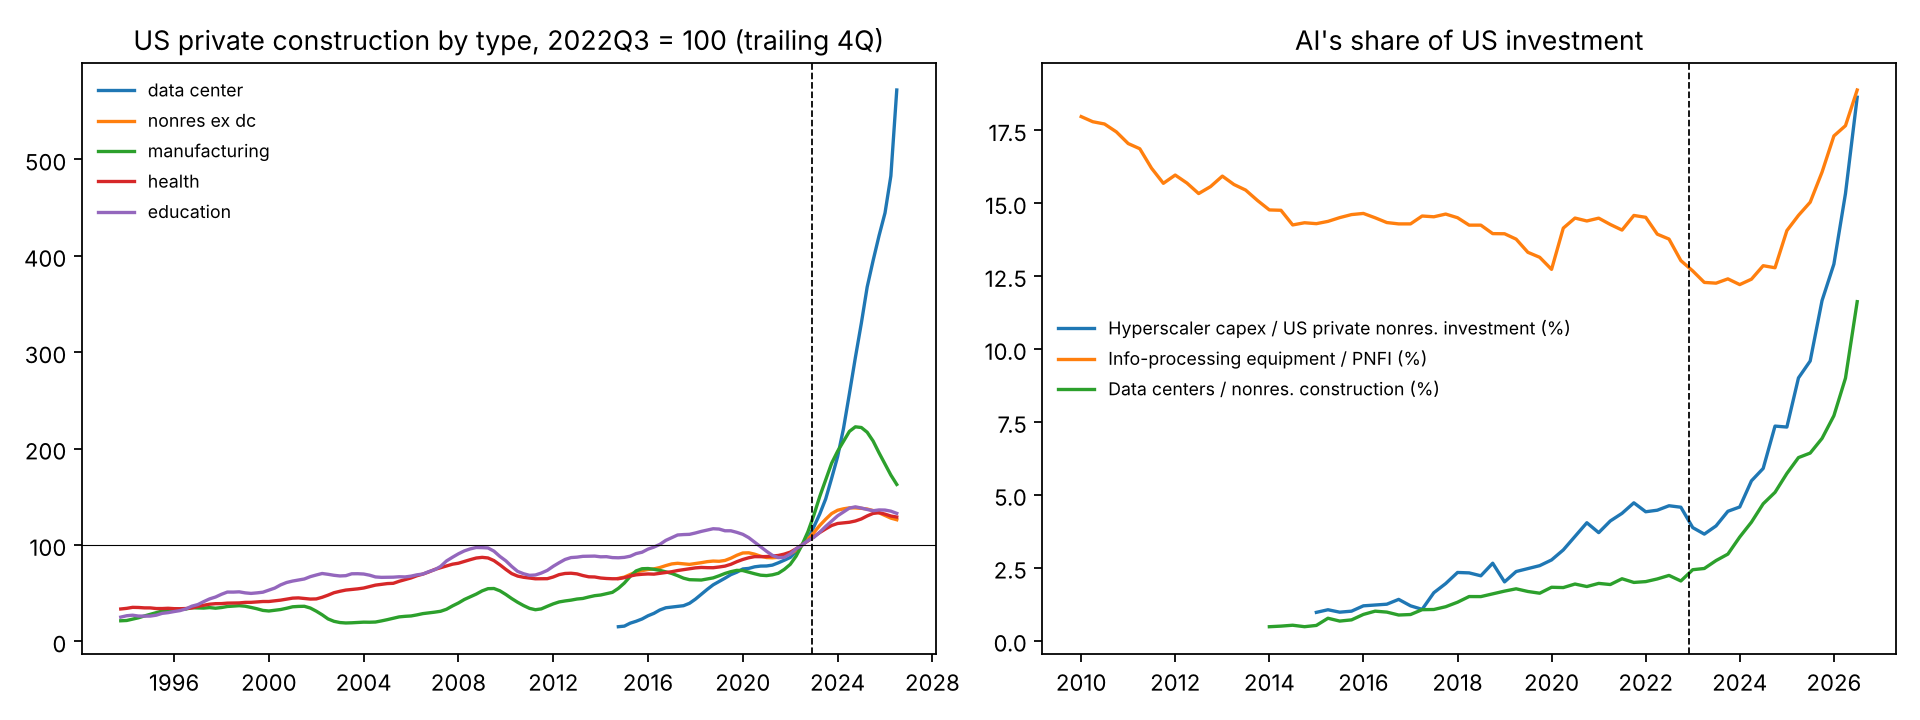
\includegraphics[width=\textwidth]{figures/fig_us_investment.png}
\caption{United States: construction by type and AI's share of investment}\label{fig:us}
\begin{figurenotes}
Left: trailing four-quarter private construction spending by category, 2022Q3 = 100 (Census Bureau). Right: hyperscaler capital expenditure as a share of private nonresidential fixed investment (BEA), information-processing equipment as a share of the same, and data-center construction as a share of private nonresidential construction. Dashed line: November 2022.
\end{figurenotes}
\end{figure}

\section{Bond markets: who is raising money}\label{sec:bonds}

The hyperscalers now fund themselves in the same international bond market as the multilateral development banks and the governments of developing countries. Table~\ref{tab:bonds} compares issuance before and after the boom, using the BIS international debt securities statistics, which cover bonds issued outside the issuer's home market.

\begin{table}
\caption{International bond issuance before and after the AI boom, USD billion per quarter}\label{tab:bonds}
\resizebox{\textwidth}{!}{\begin{tabular}{lrrr}
\toprule
Issuer & 2019Q1--2022Q3 & 2023Q1--2026Q2 & Change \\
\midrule
International organisations (IFIs), gross & 129.0 & 185.8 & +44\% \\
International organisations (IFIs), net & 40.3 & 69.9 & +73\% \\
Emerging and developing economies, all issuers, gross & 112.2 & 141.9 & +26\% \\
Emerging and developing economies, governments, gross & 49.7 & 63.2 & +27\% \\
Emerging and developing economies, governments, net & 29.6 & 32.5 & +10\% \\
Africa and Middle East governments, net & 14.8 & 12.4 & $-$16\% \\
Emerging and developing economies, nonfinancial corporations, net & 10.4 & 4.4 & $-$58\% \\
United States residents, net & 8.5 & 47.7 & +463\% \\
World, all issuers, gross & 1,678.8 & 2,097.3 & +25\% \\
\midrule
Hyperscalers, long-term debt issued (EDGAR) & 4.9 & 14.5 & +197\% \\
\bottomrule
\end{tabular}}
\begin{tablenotes}
BIS international debt securities, quarterly averages. International organisations comprise the World Bank group, the regional development banks, the European Investment Bank and other supranationals; the BIS does not publish issuer-level detail. The hyperscaler line is from Table~\ref{tab:hyp}.
\end{tablenotes}
\end{table}

Three features stand out. First, the international financial institutions are borrowing far more, not less: USD 841 billion gross over the four quarters to mid-2026, their stock of international bonds outstanding having doubled from USD 1.6 trillion at the end of 2019 to USD 3.2 trillion, and their share of world issuance having risen from about 7 to 9 percent. This is the result of the capital-adequacy reforms that allowed the multilateral banks to lever their callable capital more aggressively, and it is possible only because their AAA paper is in nearly unlimited demand from institutions that must hold safe assets. Second, emerging-market sovereigns as a group also issued more, with their outstanding stock rising 63 percent; the exceptions are Africa and the Middle East, where net sovereign issuance fell 16 percent, and nonfinancial corporations in developing economies, whose net issuance fell by more than half. Third, the growth of claims has outpaced the growth of real investment. The world stock of international bonds rose 42 percent in nominal terms while the investment rate of low-income countries fell from 24.3 to 20.9 percent of GDP; US nonfinancial corporate bonds, meanwhile, fell from 32 to 28 percent of GDP, so the expansion is not a generalized rise in leverage but the enlargement of a few balance sheets, those of development banks, sovereigns and, lately, the hyperscalers. Figure~\ref{fig:bonds} shows the time paths.

\begin{figure}
\centering
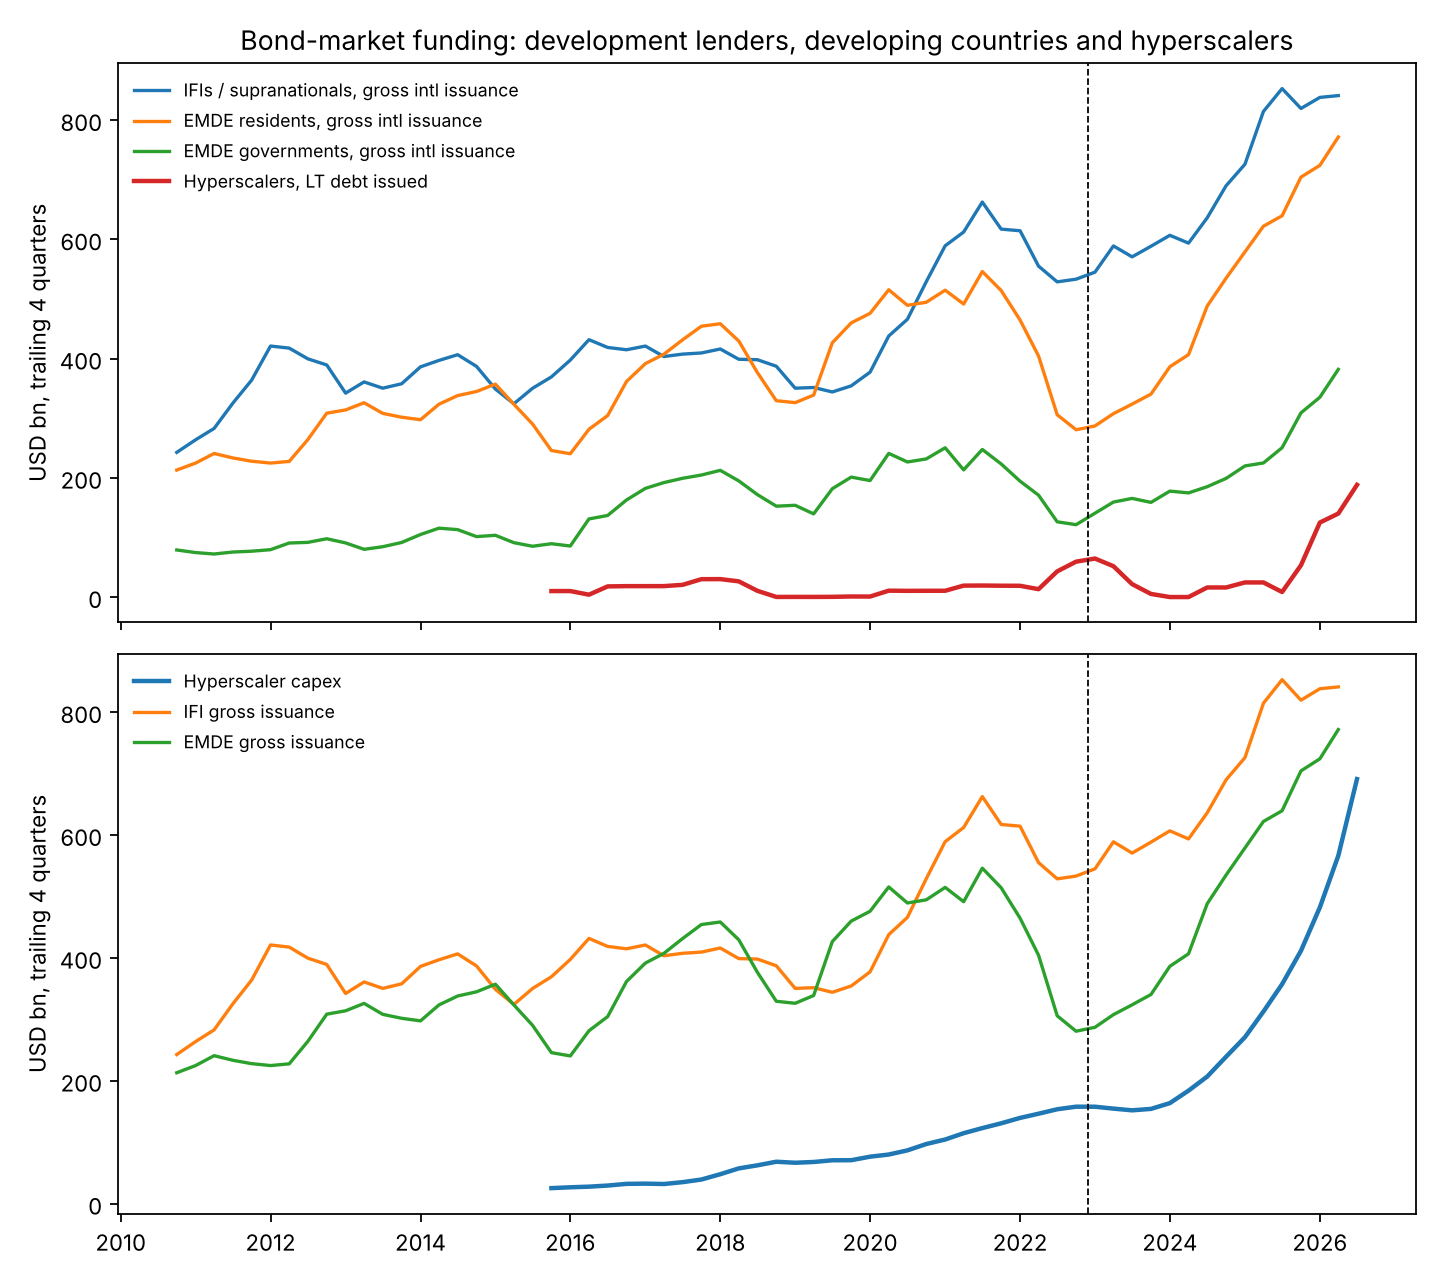
\includegraphics[width=\textwidth]{figures/fig_bond_issuance.png}
\caption{Bond-market funding of development lenders, developing countries and hyperscalers}\label{fig:bonds}
\begin{figurenotes}
Trailing four-quarter sums, USD billion. International debt securities from the BIS; hyperscaler debt and capex from EDGAR. Dashed line: November 2022.
\end{figurenotes}
\end{figure}


\begin{figure}
\centering
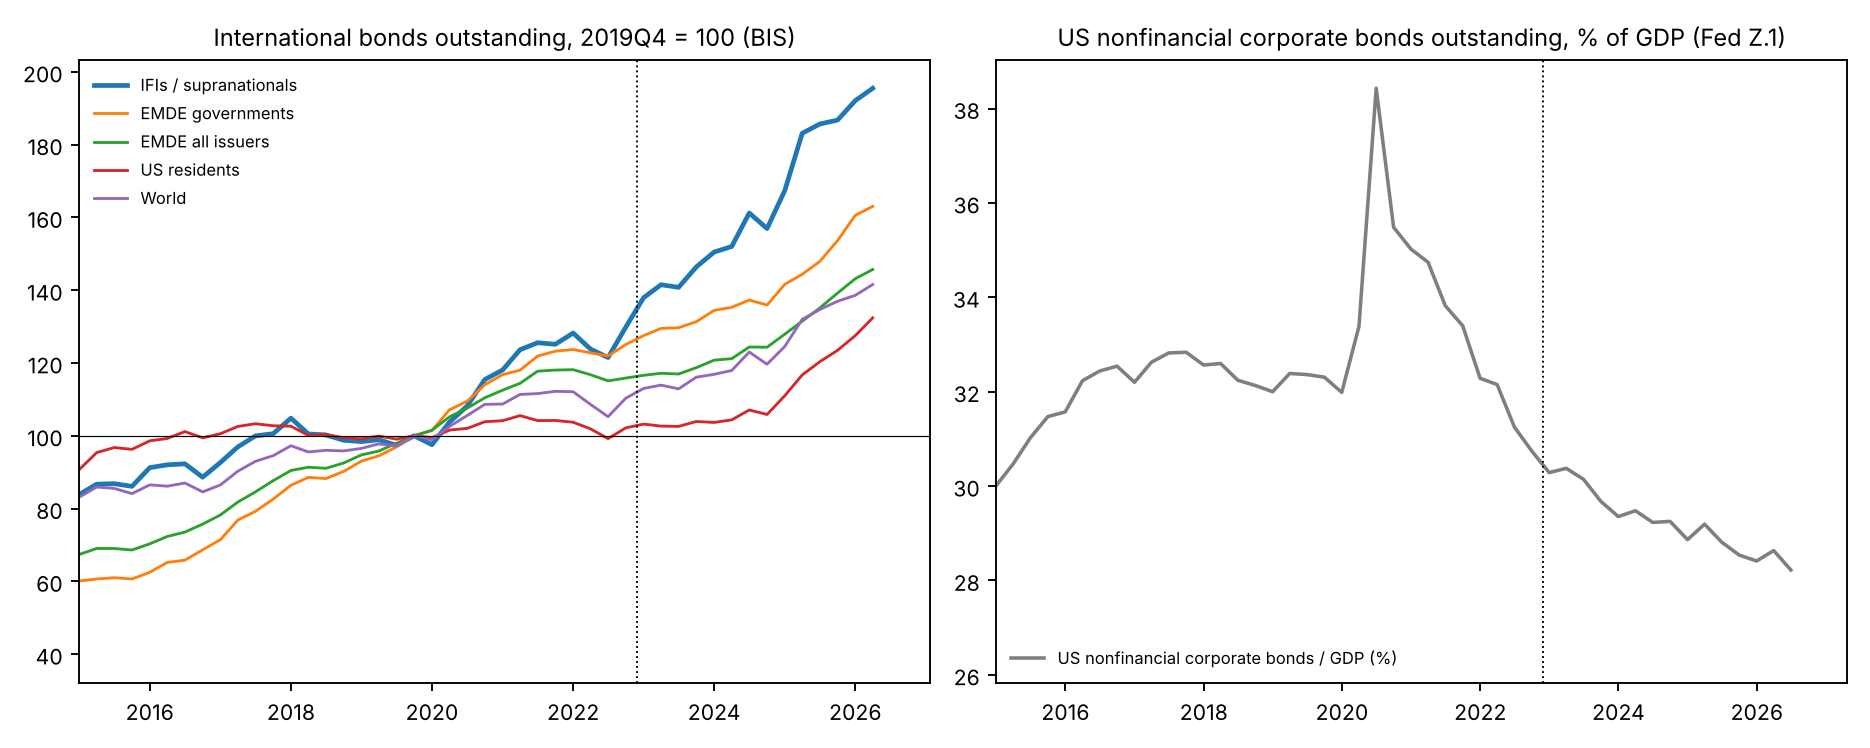
\includegraphics[width=\textwidth]{figures/fig_bond_stocks.png}
\caption{Stocks of bonds outstanding: supranationals, developing economies, the United States and the world}\label{fig:stocks}
\begin{figurenotes}
Left: international debt securities outstanding by residence of issuer, 2019Q4 = 100 (BIS). Right: US nonfinancial corporate debt securities outstanding as a share of GDP (Federal Reserve financial accounts). Dotted line: November 2022.
\end{figurenotes}
\end{figure}
Figure~\ref{fig:stocks} shows the stocks: the supranationals' outstanding bonds have nearly doubled since 2019 while US nonfinancial corporate bonds have fallen relative to GDP.

Cross-border bank lending tells the same story. BIS locational statistics show FX-adjusted flows to emerging and developing economies of USD 66 billion a quarter after 2023 against USD 9 billion before, with Africa and the Middle East receiving USD 31 billion a quarter against 12 billion, and Latin America and emerging Europe moving from net repayment to net inflow. Flows to the United States rose as well, from 104 to 237 billion a quarter. Quarterly regressions of these quantities on the AI factor give positive coefficients: quarters of high AI abnormal returns are quarters in which development banks and emerging-market sovereigns issue more, the risk-on co-movement dominating any reallocation at this frequency.

\section{Prices: do AI return shocks raise the cost of capital of developing countries?}\label{sec:prices}

If a common hurdle rate were rising with the return to AI, it should be visible in the spreads at which developing countries borrow on the days when the market learns about AI returns. Table~\ref{tab:prices} summarizes the announcement-day tests. The outcome is the two-day change in an emerging-market spread or the two-day return on an emerging-market bond fund around the 107 reaction days on which at least one of the eight AI firms reported, with the two-year Treasury yield, the VIX, the dollar, the S\&P 500 and a Treasury fund as controls.

\begin{table}
\caption{Emerging-market pricing on AI earnings days}\label{tab:prices}
\resizebox{\textwidth}{!}{\begin{tabular}{llrrr}
\toprule
Shock & Outcome & Coefficient & (s.e.) & $n$ \\
\midrule
AI firms' abnormal return & EM USD sovereign bond ETF return (\%) & $-0.10$ & (0.42) & 106 \\
AI firms' abnormal return & EM public-sector spread (bp) & 0.4 & (3.5) & 74 \\
Hyperscalers' abnormal return & EM public-sector spread (bp) & $-8.9$ & (4.3) & 44 \\
Capex surprise (\% of assets) & EM local-currency bond ETF return (\%) & $-8.6$ & (3.3) & 97 \\
Capex surprise (\% of assets) & EM high-yield bond ETF return (\%) & $-7.6$ & (4.0) & 97 \\
Capex surprise (\% of assets) & EM public-sector spread (bp) & 67.0 & (38.0) & 69 \\
Capex surprise (\% of assets) & US high-yield spread (bp), placebo & 148.7 & (63.4) & 69 \\
Supplier-implied capex shock & EM public-sector spread (bp) & $-18.1$ & (17.1) & 44 \\
\bottomrule
\end{tabular}}
\begin{tablenotes}
Two-day windows starting on the first session after the release. Abnormal returns are from a Fama--French five-factor model with momentum; the capex surprise is realized capex minus a seasonal random walk with drift, scaled by lagged assets (one standard deviation is about 0.01); the supplier-implied shock is the abnormal return of the AI supply-chain basket on hyperscaler announcement days. All regressions include the controls listed in the text. HAC standard errors. ICE BofA spread series are available on FRED only from November 2023.
\end{tablenotes}
\end{table}


\begin{figure}
\centering
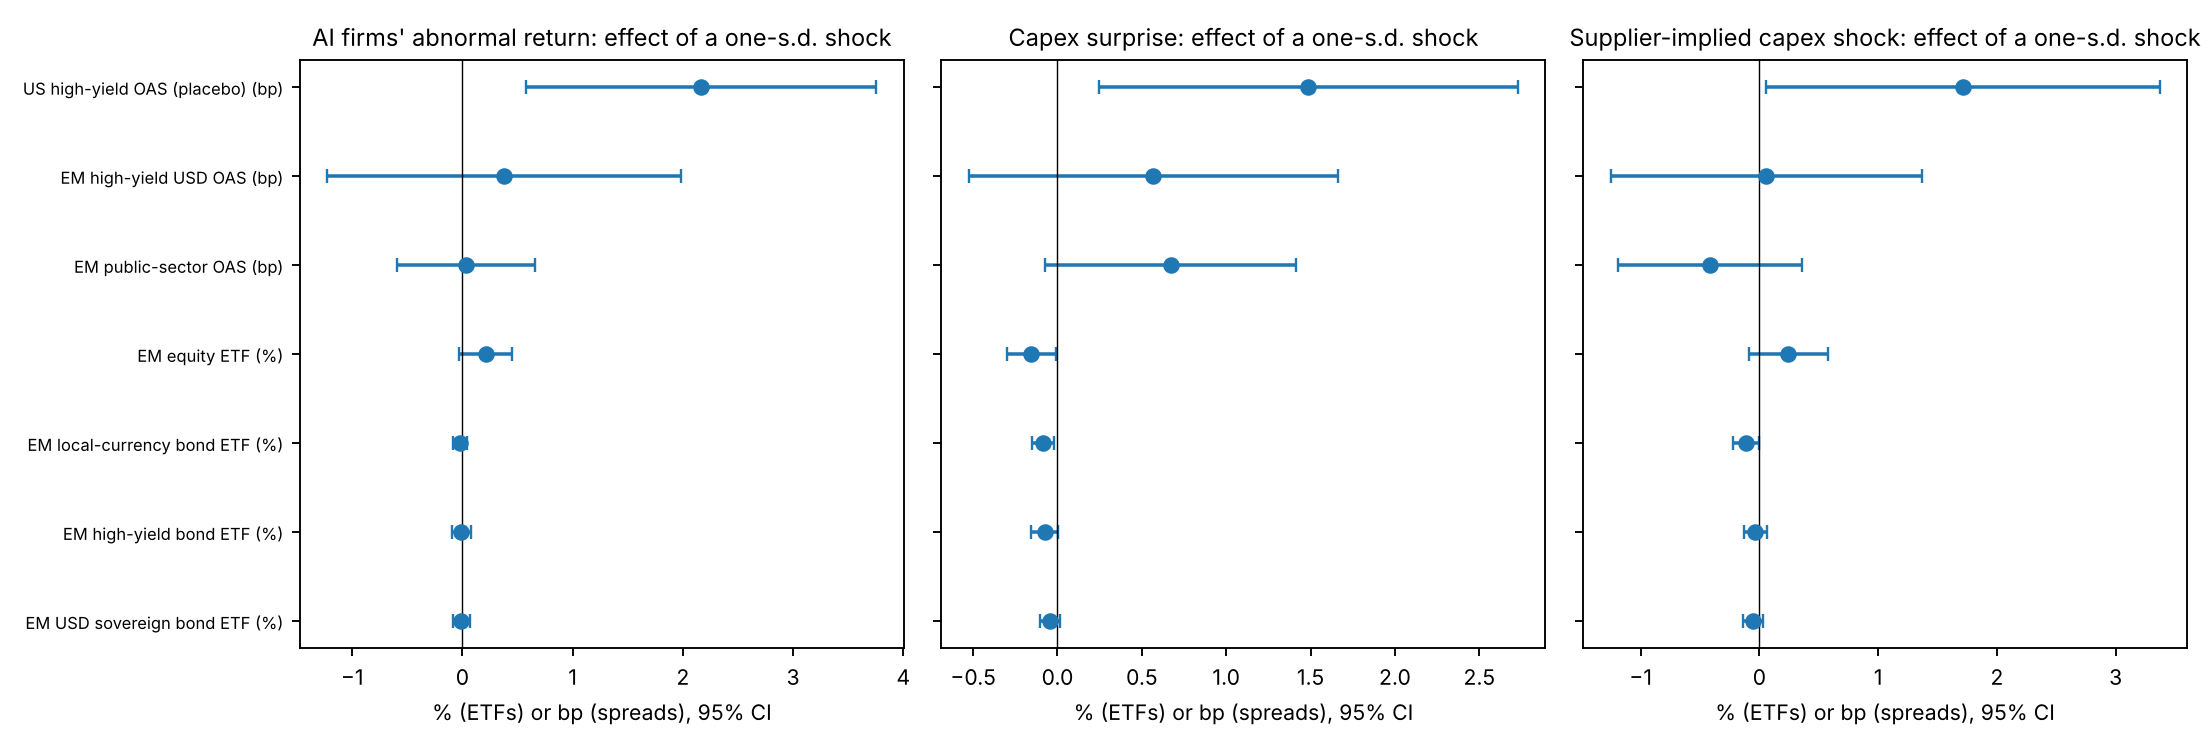
\includegraphics[width=\textwidth]{figures/fig_event_coefs.png}
\caption{Announcement-day responses of emerging-market assets to AI shocks}\label{fig:coefs}
\begin{figurenotes}
Coefficients from the regressions in Table~\ref{tab:prices} rescaled to a one-standard-deviation shock, with 95 percent confidence intervals (HAC). Outcomes are two-day ETF returns in percent or two-day spread changes in basis points.
\end{figurenotes}
\end{figure}
Figure~\ref{fig:coefs} plots the same coefficients scaled to one-standard-deviation shocks. Abnormal returns of the AI firms, the market's revision of expected AI cash flows, do not move emerging-market spreads; if anything, hyperscaler surprises come with marginally tighter spreads. The daily AI factor co-moves positively with emerging-market assets, and the co-movement disappears once the market return is controlled for. The capital-expenditure surprise is the one shock with the predicted sign: a one-standard-deviation surprise lowers emerging-market bond funds by about 0.1 percent and raises the emerging-market public-sector spread by about 0.7 basis points. But US high-yield spreads widen by twice as much on the same days, so the response is a general repricing of risk rather than one specific to developing countries, and it is small. Figure~\ref{fig:aiem} shows that over the whole period the cumulative abnormal return of the AI basket and the price of emerging-market sovereign debt rose together while emerging-market spreads fell from 200 to 115 basis points.

\begin{figure}
\centering
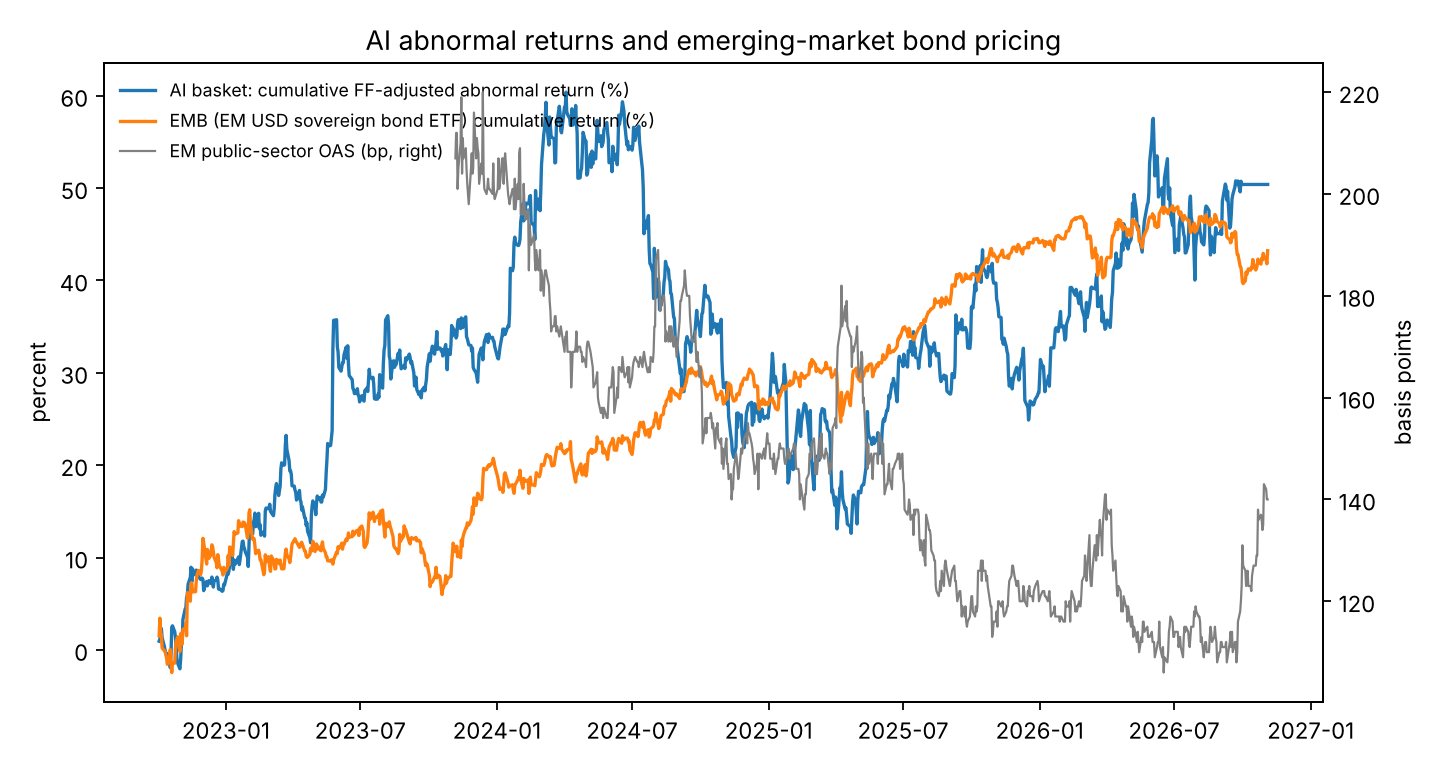
\includegraphics[width=\textwidth]{figures/fig_ai_factor_vs_em.png}
\caption{AI abnormal returns and emerging-market bond pricing}\label{fig:aiem}
\begin{figurenotes}
Cumulative Fama--French-adjusted abnormal return of the AI basket, cumulative return of the iShares J.P. Morgan USD EM bond ETF, and the ICE BofA emerging-market public-sector OAS (right axis).
\end{figurenotes}
\end{figure}

\section{Development assistance: donors}\label{sec:donors}

Table~\ref{tab:oda} reports net ODA by donor in constant prices. The DAC total rose from USD 170 billion in 2018 to a peak of 232 billion in 2023, fell 8 percent in 2024, and fell a further 23 percent in 2025 to 163 billion, below its 2019 level. The United States accounts for USD 37 billion of the 49 billion decline in 2025; its ODA fell 57 percent. Germany, Japan, France, the United Kingdom and the Netherlands cut by between 5 and 21 percent; Canada, Spain, Italy and Sweden increased. Excluding the United States, DAC ODA fell 8 percent in 2025 and 19 percent from its 2023 peak.

\begin{table}
\caption{Net ODA by donor, constant USD billion}\label{tab:oda}
\resizebox{\textwidth}{!}{\begin{tabular}{lrrrrrrrr}
\toprule
 & 2018 & 2019 & 2020 & 2021 & 2022 & 2023 & 2024 & 2025 \\
\midrule
DAC total & 169.5 & 168.1 & 181.0 & 193.6 & 229.9 & 232.1 & 212.5 & 163.1 \\
United States & 41.4 & 39.8 & 42.1 & 54.1 & 64.1 & 66.1 & 65.3 & 28.3 \\
Germany & 29.4 & 28.5 & 33.5 & 34.8 & 41.2 & 42.5 & 33.2 & 26.2 \\
United Kingdom & 23.5 & 23.8 & 22.5 & 17.6 & 18.0 & 19.8 & 16.3 & 15.3 \\
France & 13.7 & 13.3 & 17.0 & 16.9 & 19.4 & 16.2 & 15.1 & 13.2 \\
Japan & 8.0 & 9.2 & 10.4 & 12.3 & 15.6 & 17.8 & 15.2 & 13.0 \\
DAC excluding United States & 128.1 & 128.3 & 138.9 & 139.5 & 165.8 & 166.1 & 147.1 & 134.8 \\
\bottomrule
\end{tabular}}
\begin{tablenotes}
OECD DAC1, net disbursements, constant 2024 prices. 2025 figures are preliminary.
\end{tablenotes}
\end{table}


\begin{figure}
\centering
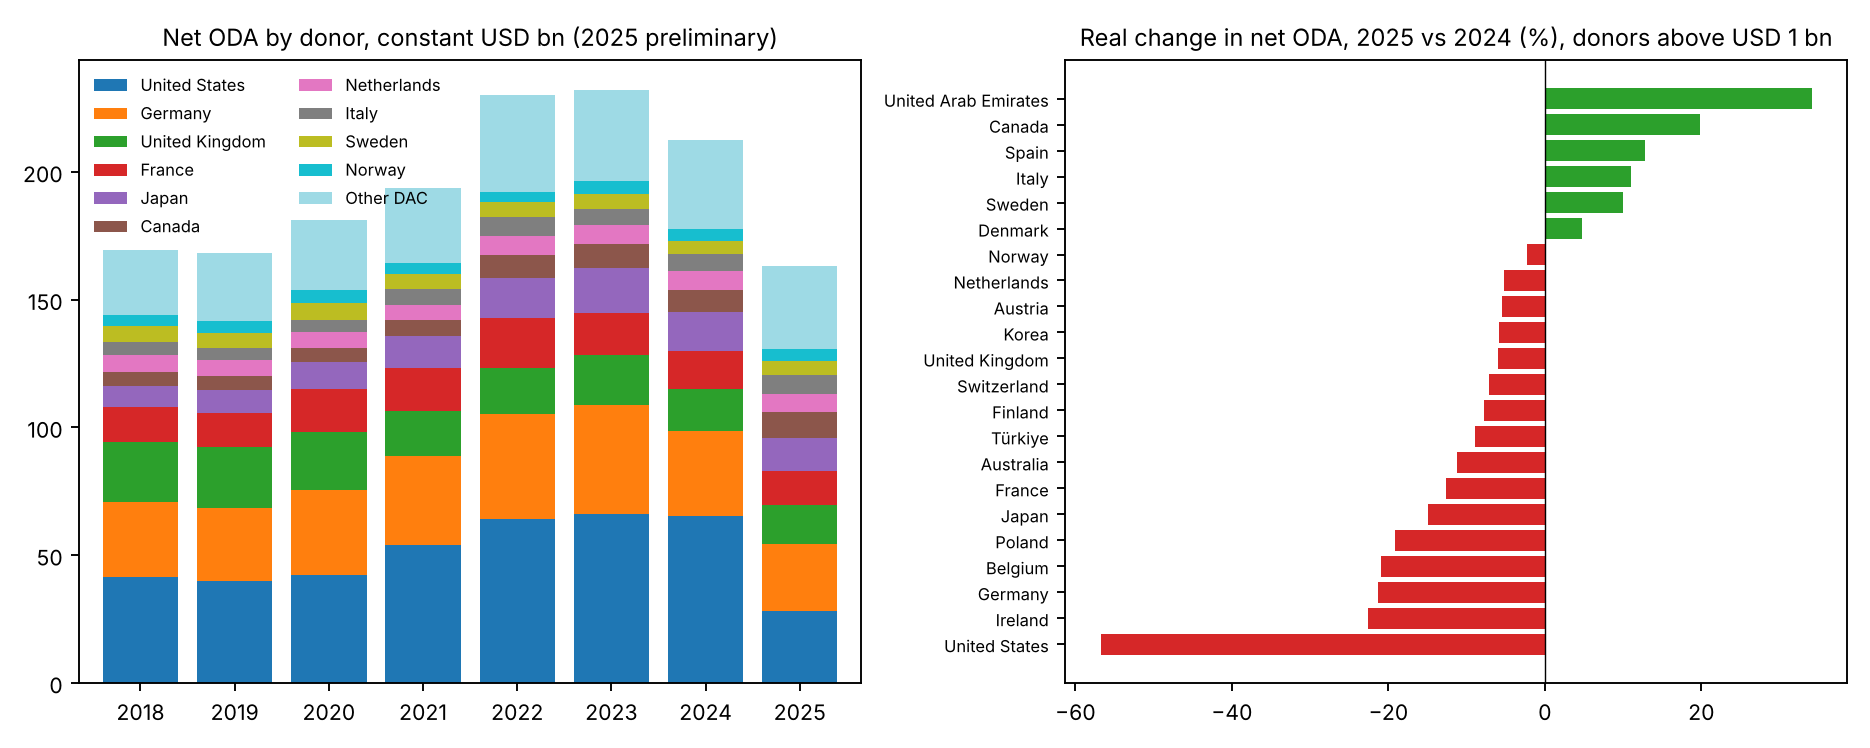
\includegraphics[width=\textwidth]{figures/fig_oda_donors.png}
\caption{Net ODA by donor and the 2025 cut}\label{fig:donors}
\begin{figurenotes}
Left: net ODA by donor, constant USD billion (OECD DAC1; 2025 preliminary). Right: real change in net ODA between 2024 and 2025 for donors above USD 1 billion.
\end{figurenotes}
\end{figure}
Figure~\ref{fig:donors} shows the donor composition and the 2025 changes.

Two parts of the earlier rise deserve note because they shape what came after. The increase between 2021 and 2023 was dominated by support to Ukraine, which rose from USD 2 billion a year to 36 billion, and by spending on refugees inside donor countries, which rose from USD 12 billion to 36 billion in 2022 before falling back to 29 billion in 2024. Neither item reaches the poorest countries, and the 2024 decline was largely the unwinding of the second.

Private finance mobilised by official development interventions, the vehicle that the companion paper's crowding-out mechanism predicts should fall first because it competes for the common pool, rose instead, to USD 297 billion in 2024 from 260 billion in 2022 and 206 billion in 2018. Its destination is instructive: USD 123 billion went to banking and financial services, 37 billion to energy, 25 billion to transport, and 1.5 and 1.8 billion to health and education. By income group, USD 37 billion was mobilised for upper-middle-income countries, 19 billion for lower-middle-income and 3 billion for low-income countries.


\begin{figure}
\centering
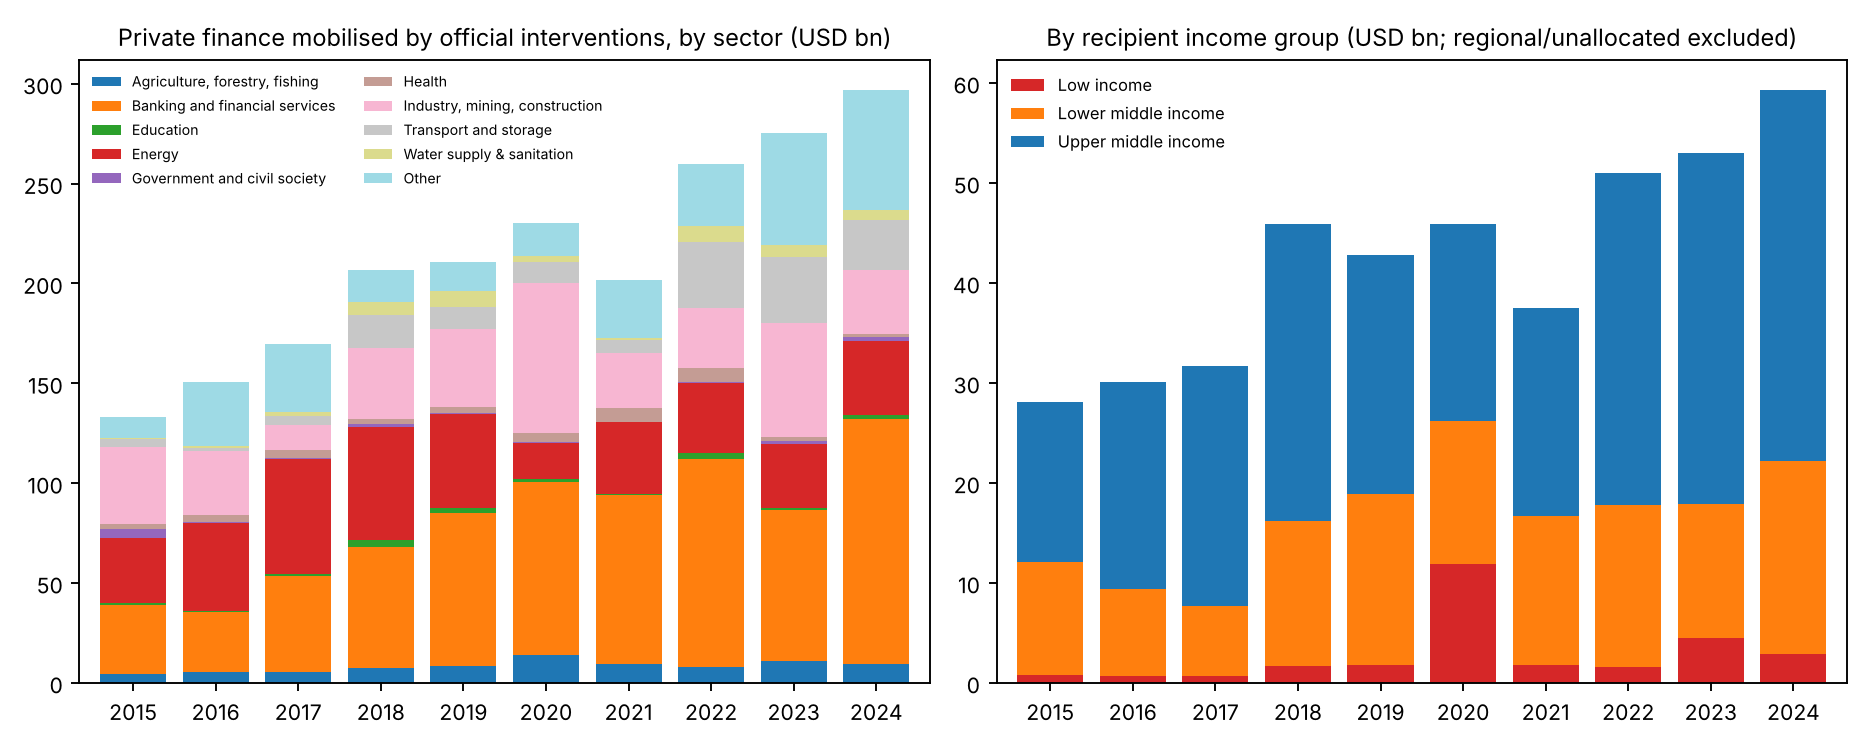
\includegraphics[width=\textwidth]{figures/fig_mobilisation.png}
\caption{Private finance mobilised by official development interventions}\label{fig:mob}
\begin{figurenotes}
Amounts mobilised from the private sector by official development finance interventions, constant USD billion, by sector (left) and by recipient income group (right; regional and unallocated amounts excluded). Source: OECD.
\end{figurenotes}
\end{figure}
Figure~\ref{fig:mob} shows the sectoral and income-group destination of mobilised finance.

\section{Recipients: regions and countries}\label{sec:recipients}

ODA received, measured from the recipient side in the DAC2A tables, rose 25 percent between 2019--21 and 2023--24 for developing countries as a whole, but Table~\ref{tab:recip} shows that the increase went almost entirely to Ukraine. Low-income countries received 12 percent less in 2023--24 than in 2019--21, before the 2025 collapse; Sub-Saharan Africa received 3 percent more; fragile contexts 3 percent less; Northern Africa and the Middle East substantially less. Upper-middle-income countries, where Ukraine is classified, received 133 percent more.

\begin{table}
\caption{ODA received by recipient group, constant USD billion}\label{tab:recip}
\resizebox{\textwidth}{!}{\begin{tabular}{lrrrrr}
\toprule
 & 2019--21 avg & 2024 & Change (\%) & US share 2024 (\%) & Humanitarian share 2024 (\%) \\
\midrule
All developing countries & 208.5 & 255.7 & +25 & 23 & 15 \\
Low income & 57.4 & 49.2 & $-$12 & 21 & 37 \\
Lower-middle income & 56.1 & 59.1 & +2 & 15 & 13 \\
Upper-middle income & 26.7 & 58.8 & +133 & 28 & 8 \\
Fragile contexts & 98.4 & 95.2 & $-$3 & 18 & 26 \\
Sub-Saharan Africa & 64.4 & 68.1 & +3 & 23 & 18 \\
Middle East & 27.8 & 22.9 & $-$12 & 16 & 53 \\
South and Central Asia & 23.5 & 23.7 & 0 & 17 & 14 \\
Ukraine & 2.1 & 35.6 & +1,595 & 27 & -- \\
\bottomrule
\end{tabular}}
\begin{tablenotes}
OECD DAC2A, net ODA disbursements from all official donors, constant prices. Change compares the 2023--24 average with the 2019--21 average. Income groups follow the World Bank classification used by the OECD.
\end{tablenotes}
\end{table}


\begin{figure}
\centering
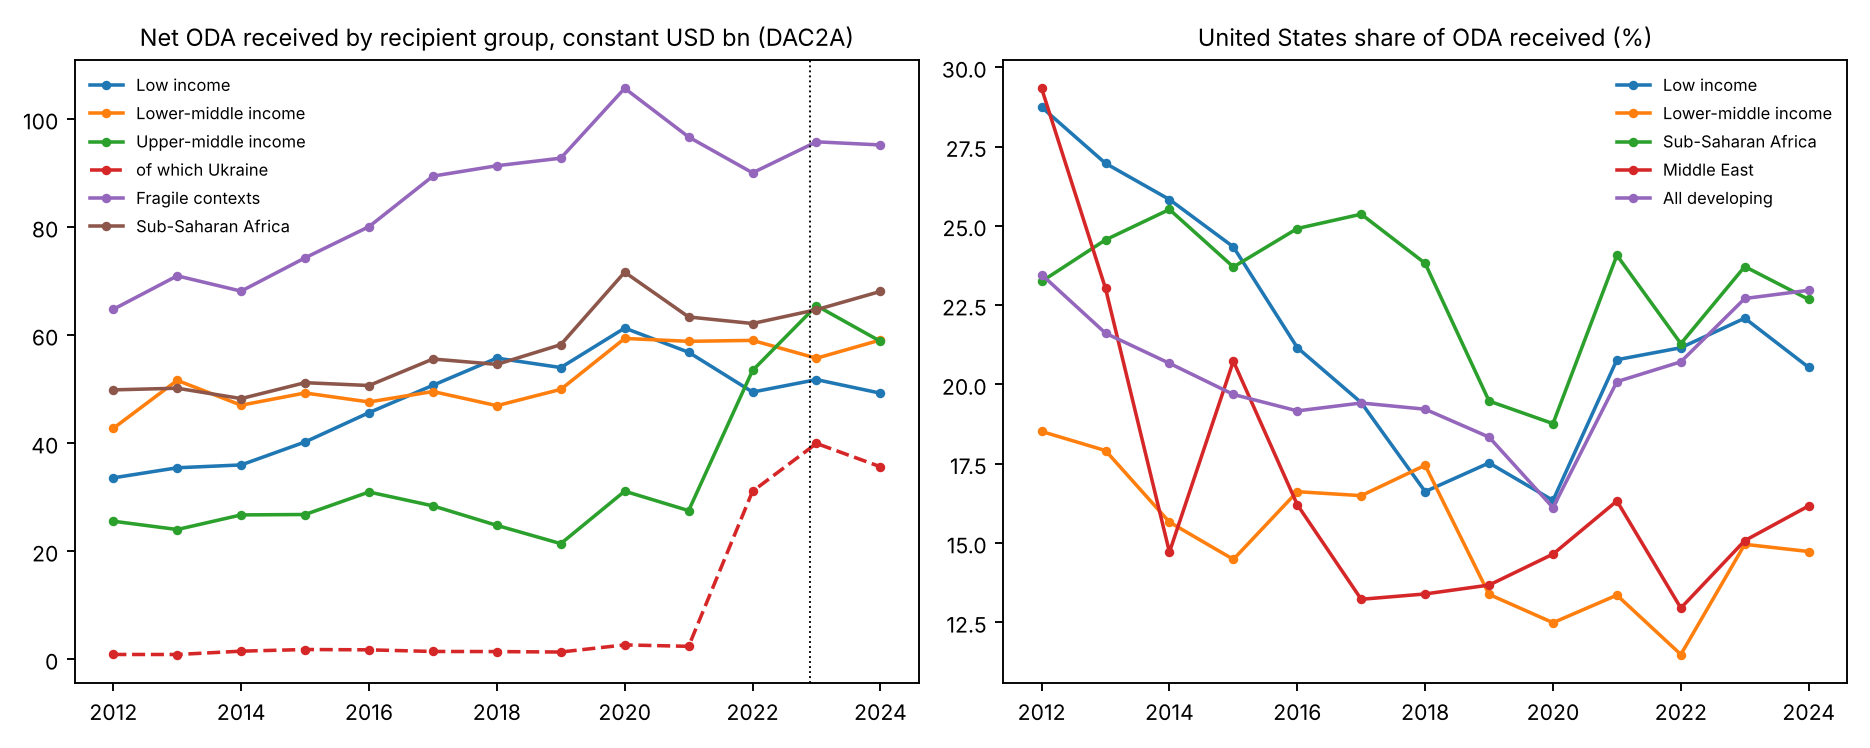
\includegraphics[width=\textwidth]{figures/fig_recipient_groups.png}
\caption{ODA received by recipient group and the United States share}\label{fig:groups}
\begin{figurenotes}
Left: net ODA received by recipient group, constant USD billion (OECD DAC2A); Ukraine shown separately. Right: share of ODA received that came from the United States. Dotted line: November 2022.
\end{figurenotes}
\end{figure}

\begin{figure}
\centering
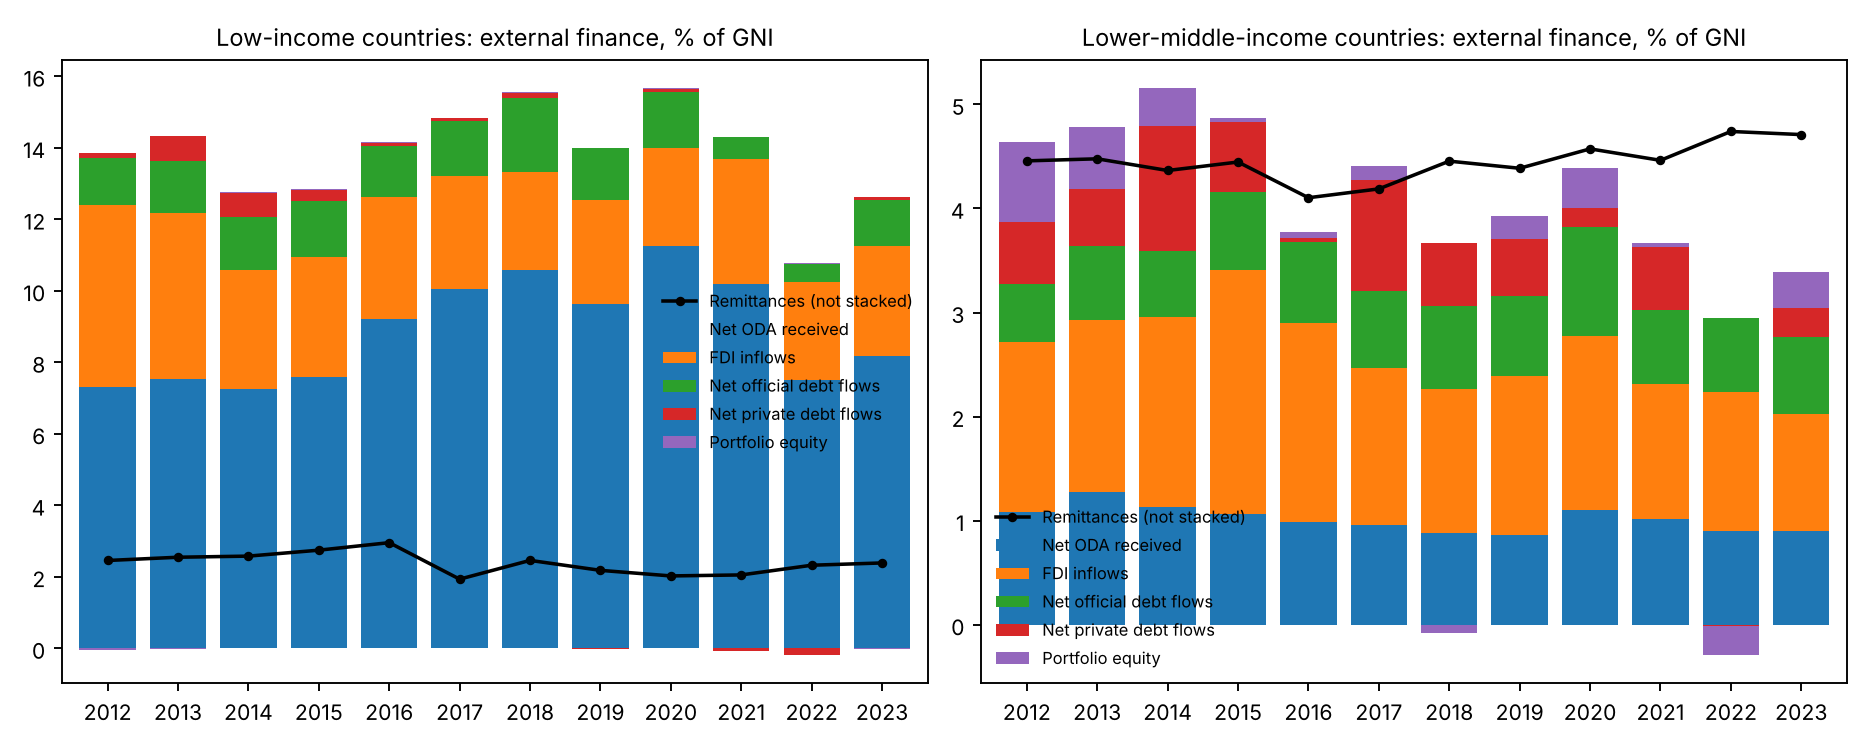
\includegraphics[width=\textwidth]{figures/fig_lic_finance.png}
\caption{External finance of low- and lower-middle-income countries, percent of GNI}\label{fig:licfin}
\begin{figurenotes}
Net ODA received, FDI inflows, net official and private external-debt flows and portfolio equity, stacked, as a percent of GNI; remittances shown as a line. Sources: World Bank WDI and IDS, income-group aggregates.
\end{figurenotes}
\end{figure}
Figure~\ref{fig:groups} shows the recipient groups over time and the US share of each, and Figure~\ref{fig:licfin} the composition of external finance for low- and lower-middle-income countries as a share of GNI: for low-income countries ODA is three-quarters of the total and private debt flows are nil.

The country-level record combines the OECD recipient data with the World Bank's external-flow and debt statistics for 131 low- and middle-income countries. For each country I compute net ODA as a share of GNI, the US share of its 2024 ODA, whether it had any access to markets in 2022--24 (any public or private bond issuance, or positive net flows from private creditors), and the change in its total external finance between 2019--21 and 2022--24. The median low-income country receives ODA equal to 8.8 percent of GNI, 22 percent of it from the United States; only 24 percent of low-income countries have market access; and their total external finance fell by 1.7 percentage points of GNI between the two periods, all of it from ODA, private flows having been unchanged at zero. The corresponding figures for lower-middle-income countries are 3.6 percent of GNI, 13 percent US share, 38 percent with market access and a 0.3-point decline.

Defining a country as left behind if ODA exceeds 5 percent of GNI and it has no market access yields 32 countries with 398 million people, 311 million of them in Sub-Saharan Africa. Applying the observed 57 percent US cut to each country's 2024 US share gives a first measure of exposure to 2025: Afghanistan loses about 3.8 percent of GNI, Somalia 3.3, Liberia 2.9, the Central African Republic 2.4, Mozambique 2.4, Lesotho 1.8, Malawi 1.7, Niger 1.5, Jordan 1.3, Haiti and Burundi 1.1, and the Democratic Republic of Congo, with 109 million people, 0.9 percent. Figure~\ref{fig:exposure} plots aid dependence against the US share for all countries; the countries without market access, marked with black edges, are concentrated where both are high.

\begin{figure}
\centering
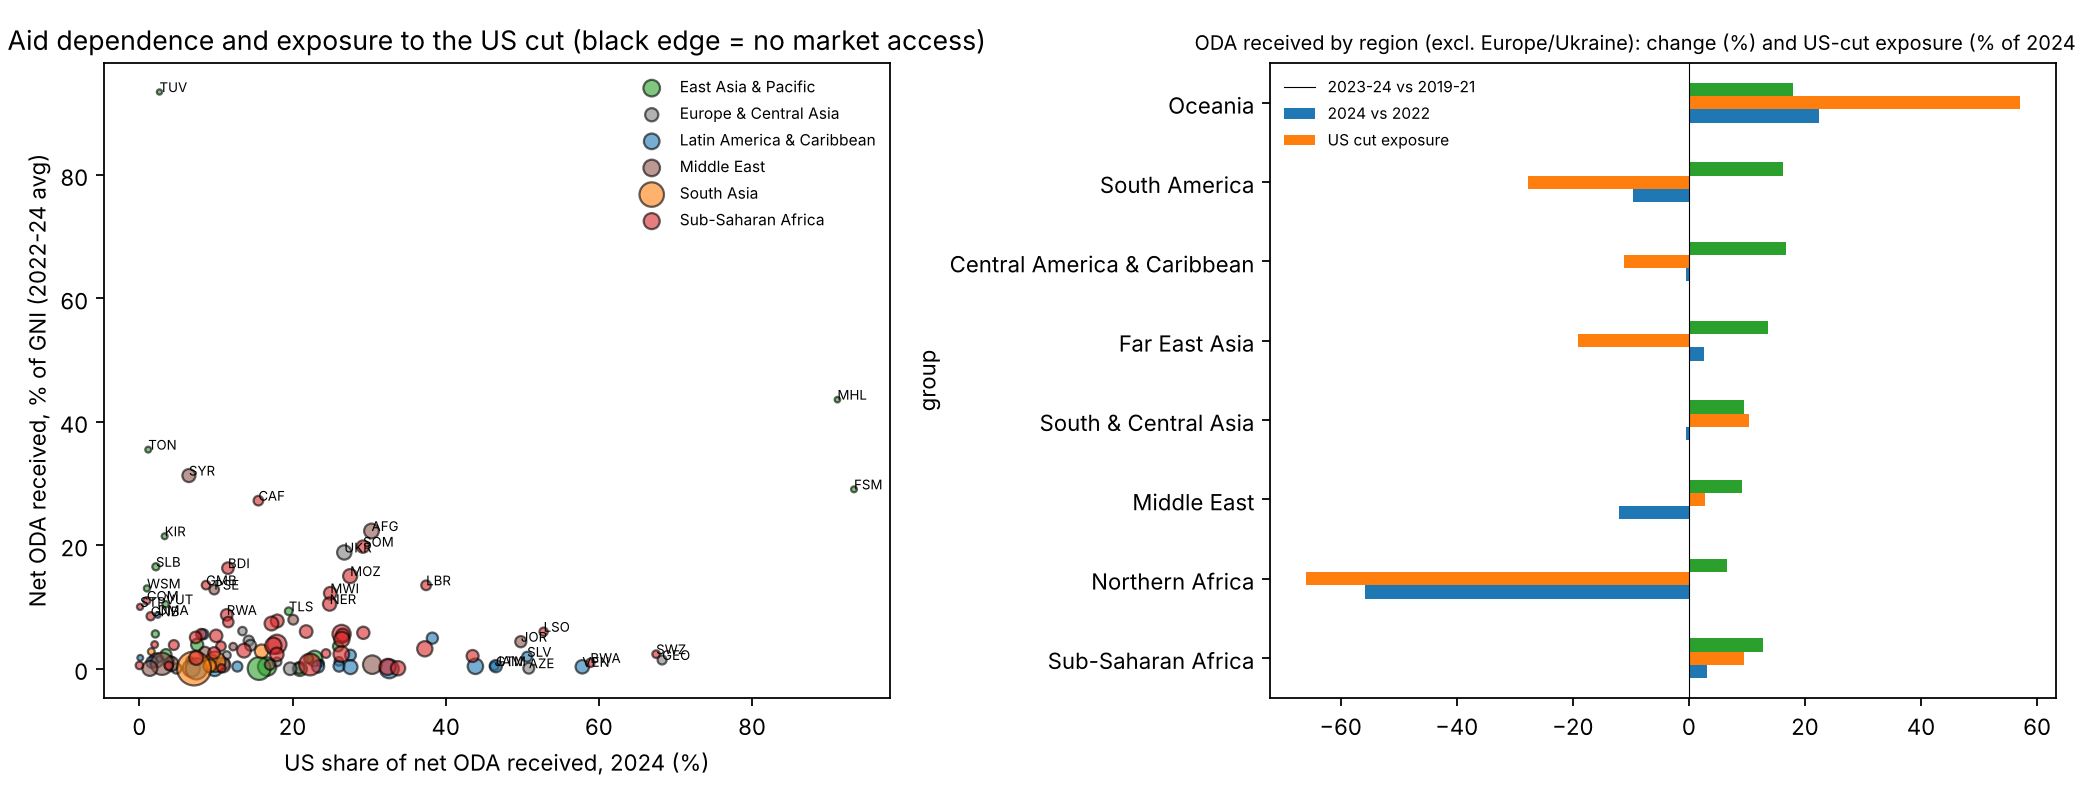
\includegraphics[width=\textwidth]{figures/fig_country_exposure.png}
\caption{Aid dependence, exposure to the US cut, and market access}\label{fig:exposure}
\begin{figurenotes}
Left: net ODA received as a share of GNI (2022--24 average) against the US share of 2024 ODA; bubble area proportional to population; black edge denotes no market access in 2022--24. Right: change in ODA received by region and exposure to the 2025 US cut as a share of 2024 ODA; Europe (Ukraine) omitted. Sources: OECD DAC2A, World Bank WDI and IDS.
\end{figurenotes}
\end{figure}


\begin{figure}
\centering
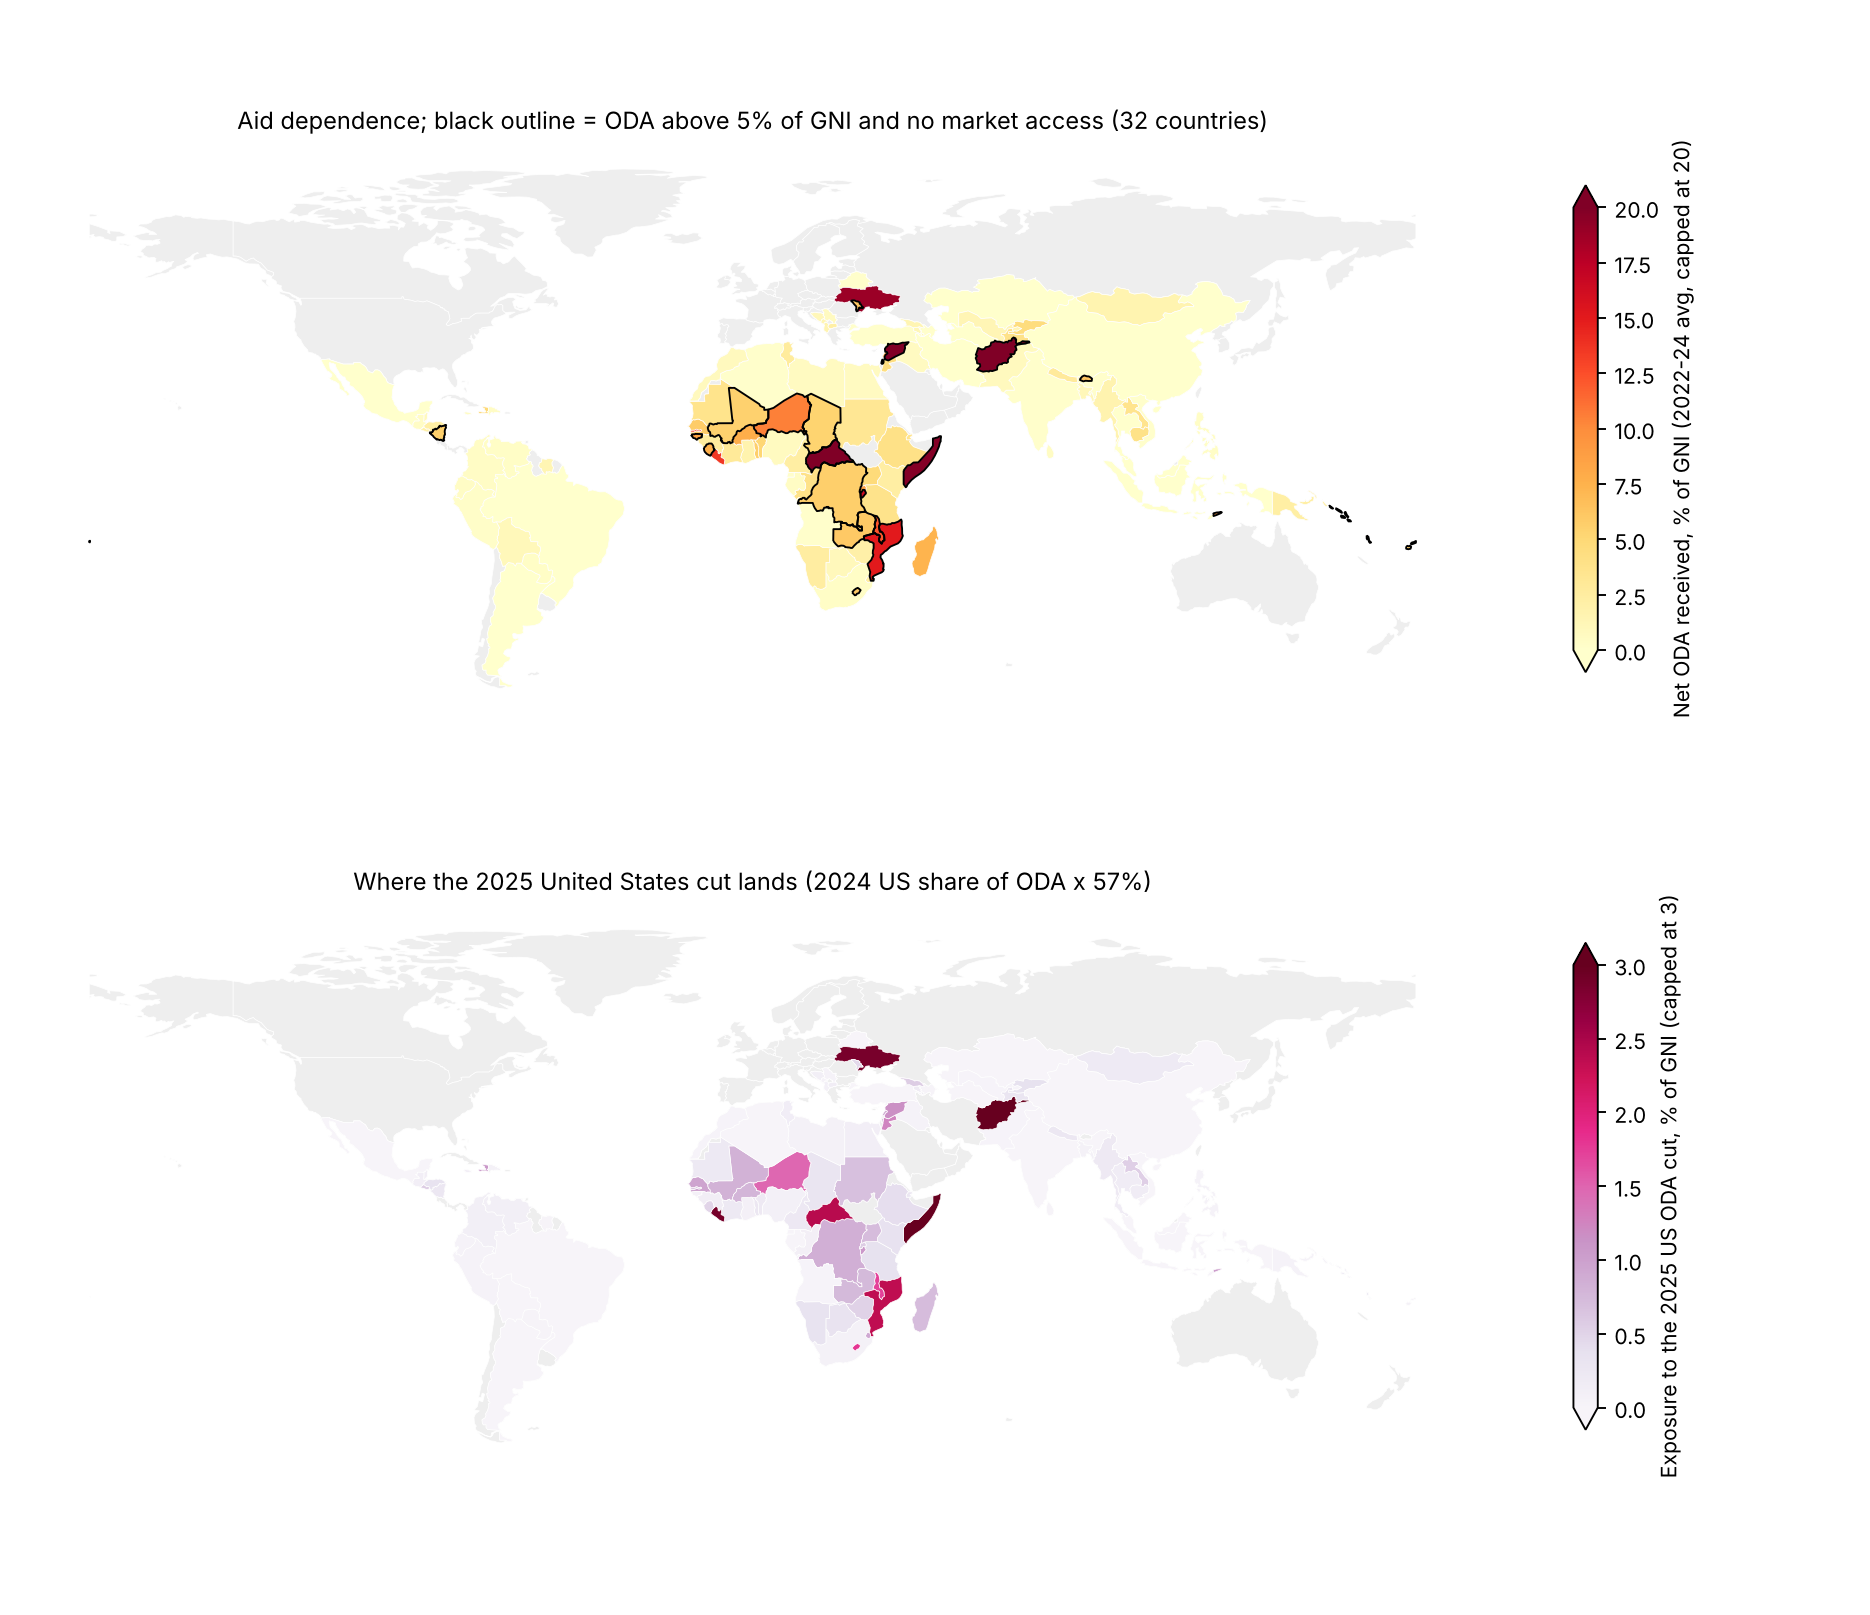
\includegraphics[width=\textwidth]{figures/fig_map_exposure.png}
\caption{Aid dependence and exposure to the 2025 US cut}\label{fig:map}
\begin{figurenotes}
Top: net ODA received as a share of GNI, 2022--24 average; black outlines mark the 32 countries with ODA above 5 percent of GNI and no market access. Bottom: exposure to the 2025 US cut, 2024 US share of ODA times 57 percent, as a share of GNI. Sources: OECD DAC2A, World Bank; boundaries from Natural Earth.
\end{figurenotes}
\end{figure}
Figure~\ref{fig:map} maps both measures.

\section{Sectors}\label{sec:sectors}

Table~\ref{tab:sectors} disaggregates ODA received by developing countries by purpose sector, from the Creditor Reporting System. Health was the largest loser before 2025: disbursements fell 40 percent between 2022 and 2024 as the pandemic response unwound and then continued to fall, to below their 2019 level. Humanitarian aid, government and civil society, and education fell modestly; the infrastructure sectors, energy, transport and water, were flat or rising; budget support, which is Ukraine, rose 59 percent.

\begin{table}
\caption{ODA received by developing countries by sector, constant USD billion}\label{tab:sectors}
\resizebox{\textwidth}{!}{\begin{tabular}{lrrrrrr}
\toprule
Sector & 2019--21 & 2022 & 2024 & Change 2024/22 (\%) & US share 2024 (\%) & US cut exposure (USD bn) \\
\midrule
Humanitarian & 38.8 & 40.9 & 38.2 & $-$7 & 34 & 7.4 \\
Budget support & 12.4 & 21.5 & 34.0 & +59 & 4 & 0.8 \\
Government and civil society & 25.2 & 32.4 & 30.5 & $-$6 & 40 & 6.9 \\
Refugees in donor countries & 11.9 & 36.5 & 28.6 & $-$22 & 24 & 4.0 \\
Health & 21.1 & 28.8 & 17.3 & $-$40 & 16 & 1.6 \\
Education & 16.3 & 17.0 & 16.6 & $-$2 & 9 & 0.9 \\
Transport & 11.3 & 13.8 & 14.1 & +2 & 1 & 0.1 \\
Population and reproductive health (incl.\ HIV/AIDS) & 10.9 & 13.3 & 13.8 & +4 & 66 & 5.1 \\
Energy & 11.7 & 13.8 & 13.5 & $-$2 & 6 & 0.4 \\
Agriculture & 10.4 & 10.7 & 10.8 & +1 & 12 & 0.7 \\
Water and sanitation & 7.3 & 7.4 & 8.1 & +9 & 7 & 0.3 \\
Environment & 5.3 & 5.0 & 7.4 & +48 & 10 & 0.4 \\
Banking and finance & 7.0 & 7.0 & 3.9 & $-$45 & 1 & 0.0 \\
\midrule
All sectors & -- & 300.3 & 289.1 & $-$4 & 20 & 33.4 \\
\bottomrule
\end{tabular}}
\begin{tablenotes}
OECD CRS, gross ODA disbursements to all developing countries from all official donors, constant prices. US cut exposure is the US 2024 disbursement in the sector times the observed 57 percent real reduction in US ODA in 2025. The ``All sectors'' row includes sectors not listed.
\end{tablenotes}
\end{table}

The composition prediction of the companion model, that capital-intensive development capital should contract by more than labour-intensive services when the hurdle rate rises, is not borne out. Grouping energy, transport, water and industry as capital-intensive and health, population, education and government services as labour-intensive, the former rose 3 percent and the latter fell 13 percent between 2022 and 2024 for all developing countries; in low-income countries the figures are +8 and $-$10 percent, and in Sub-Saharan Africa +7 and $-$7 percent. The ordering is reversed in every group except lower-middle-income countries, where it is weak. The 2025 cut sharpens the reversal: the United States funded 66 percent of population and reproductive health (where HIV programmes are classified), 40 percent of government and civil society, 34 percent of humanitarian relief and 16 percent of health, against 1 to 7 percent of transport, energy and water. The sector-level exposure to the US cut is USD 33 billion, 12 percent of ODA to developing countries, of which 7.4 billion falls on humanitarian relief, 6.9 billion on government services, 5.1 billion on HIV and reproductive health and 1.6 billion on other health. Figure~\ref{fig:sectors} shows the sector composition over time and the US share by sector.

\begin{figure}
\centering
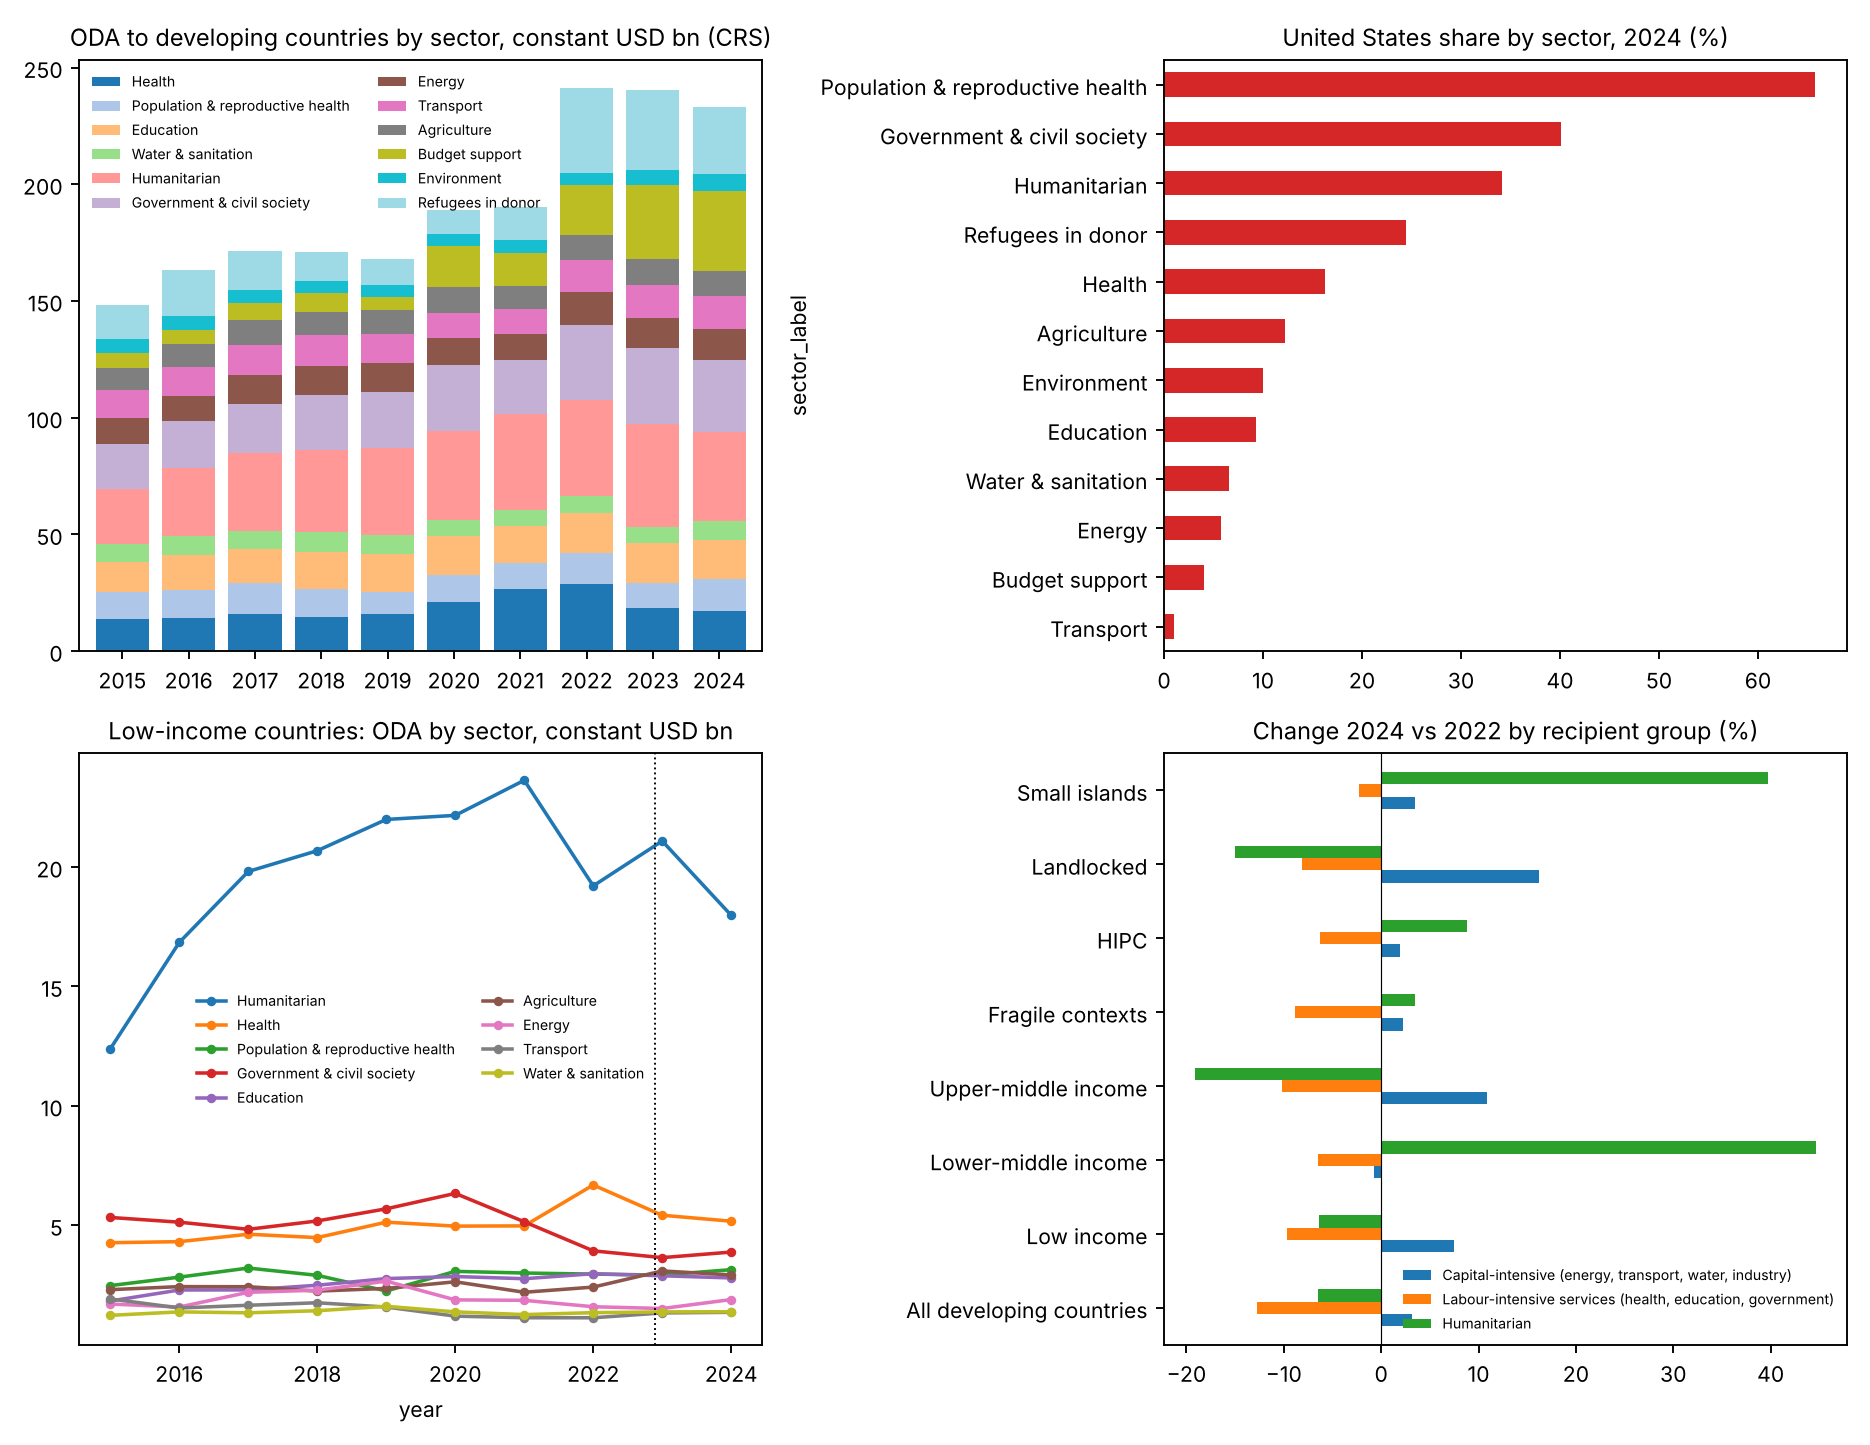
\includegraphics[width=\textwidth]{figures/fig_sectors.png}
\caption{ODA by sector, the US share, and the composition change by recipient group}\label{fig:sectors}
\begin{figurenotes}
Top left: gross ODA disbursements to developing countries by sector, constant USD billion (OECD CRS). Top right: US share of each sector in 2024. Bottom left: ODA to low-income countries by sector. Bottom right: change between 2022 and 2024 in capital-intensive sectors, labour-intensive services and humanitarian aid, by recipient group.
\end{figurenotes}
\end{figure}

At the country level the two left-behind profiles lose in different sectors. The Southern and Eastern African countries with high HIV burdens lose health: the US cut to health and HIV programmes alone amounts to about 1.6 percent of GNI in Mozambique, 1.1 in Lesotho, 1.0 in Malawi, 0.9 in Eswatini and Liberia, 0.7 in Burundi, 0.6 in Zambia and 0.5 in Uganda. The conflict economies lose humanitarian relief, of which the United States funded 65 percent in Somalia, 59 percent in Zimbabwe, 53 percent in the Democratic Republic of Congo and 44 percent in Afghanistan. Education, water and infrastructure, being funded mainly by European donors and the multilateral banks, are barely exposed. Figure~\ref{fig:csector} decomposes the exposure of the 25 most exposed countries by sector.

\begin{figure}
\centering
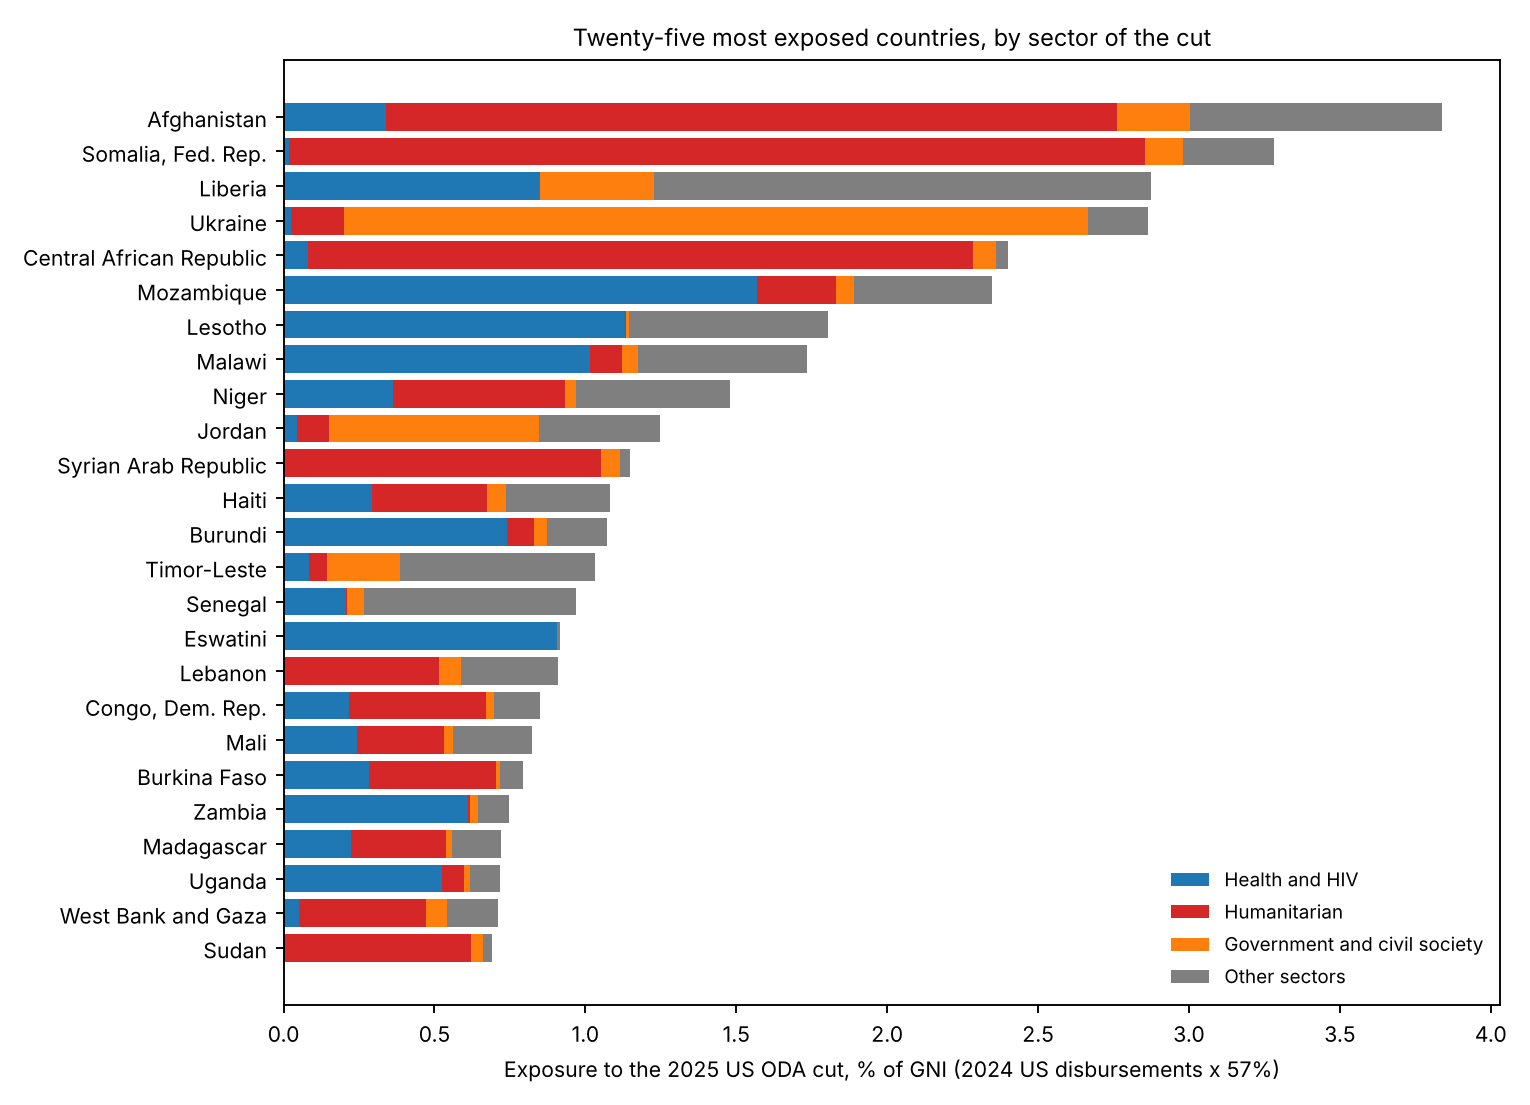
\includegraphics[width=\textwidth]{figures/fig_country_sector_exposure.png}
\caption{Exposure to the 2025 US cut by sector, 25 most exposed countries}\label{fig:csector}
\begin{figurenotes}
Exposure is the 2024 US disbursement in each sector times 57 percent, as a share of GNI (OECD CRS, World Bank). Health and HIV combines the CRS health and population/reproductive-health sectors. Compact-of-Free-Association recipients (Marshall Islands, Micronesia, Palau) are excluded because their US funding was not cut.
\end{figurenotes}
\end{figure}


\section{Interpretation}\label{sec:interp}

The companion paper sets out three explanations of the coincidence between the AI boom and the fall in development finance: a common hurdle rate that rises with the return to AI and bids capital away from poorly appropriable uses; donor politics independent of AI; and an AI-for-development effect in which AI raises the productivity of investment in poor countries. It states the implications of each for the response of development finance to AI return shocks, for the composition of the decline across vehicles and sectors, and for the cost of capital faced by low-income countries. The facts assembled here can be read against those implications.

The price evidence is null to risk-on. AI return shocks do not raise, and if anything slightly lower, the spreads at which developing countries borrow; the capex surprise raises them, but raises US high-yield spreads by as much, and the effect is a fraction of a basis point per standard deviation. The composition of the decline across vehicles is the reverse of the crowding-out prediction: the return-seeking vehicles that compete for the common pool, mobilised private finance, cross-border bank lending, sovereign Eurobonds and the borrowing of development banks, all grew, while grant budgets fell. The composition across sectors is also the reverse: capital-intensive infrastructure held up and labour-intensive services fell. Across donors, the decline is concentrated in one donor whose cut was a political decision taken in a single year, and the donors with the largest AI-exposed capital markets after the United States, the United Kingdom and Canada, cut least or increased. On the criteria the companion paper itself lays down, the 2025 collapse fits the donor-politics explanation better than the crowding-out explanation, and the AI-for-development explanation, which predicts lower spreads and more finance for sectors where AI applications are advanced, is not distinguishable from general risk appetite in these data.

Two qualifications keep the crowding-out channel open. The first is timing. The hyperscalers funded their expansion from cash flow until the third quarter of 2025 and began drawing on external capital only in the fourth; the period in which they could have competed with anyone for funds has lasted a year, and most of the post-2023 comparison predates it. The second is that ODA is the one vehicle whose funder is a government rather than an investor, so that the ``required return'' on it is political rather than a market price, and the companion model's parameter $\phi$ for grant aid measures what donor governments need to justify the allocation. A government that observes its own corporate sector investing USD 700 billion a year in AI and its own capital-gains revenue rising with AI valuations may require more of its aid budget, or less; that is an empirical question that the donor cross-section can address once donor-level AI exposure is measured.

What the facts suggest more strongly than either explanation is a reframing. There has been no scarcity of capital. The stock of financial claims grew faster than real investment everywhere, and most of all on the balance sheets that issue safe or contracted paper. The financial system allocated this abundant capital to AAA development-bank bonds, to cloud capacity with contracted revenue, to middle-income sovereign Eurobonds, and, within development finance, to the financial intermediaries and energy projects that absorb mobilised private finance. What it did not allocate to, and what contracted, is the financing of health, humanitarian relief and the functioning of governments in countries that cannot borrow, because those uses generate no return that any funder can collect. In the language of the companion model, the elasticity of the pool is high and the appropriability parameter is doing all the work: the uses with $\phi$ near zero are the ones that lost, and they lost not because funds were bid away but because the only vehicle that finances them is a grant whose provision is at the discretion of a handful of governments. The model's elastic-pool case, in which crowding out of development capital is weak but the skill premium rises more through capital deepening and the welfare cost depends on appropriability, is the case the data select, and the policy margin it points to is the one that raises $\phi$, guarantees, outcome contracts and multilateral de-risking, rather than the one that separates pools.

\section{Conclusion}

Capital expenditure on artificial intelligence by five firms now exceeds the entire stock of annual development assistance by a factor of four and, since late 2025, is financed on the same international bond market on which the development banks and the governments of developing countries borrow. That market shows no sign of scarcity: everyone with collectable returns raised more. The financing that collapsed is grant aid for services with no collectable return, in the countries that cannot replace it, delivered through the sectors, HIV programmes, humanitarian relief and government services, that one donor had come to dominate. Thirty-two countries with 400 million people, three-quarters of them in Sub-Saharan Africa, depend on this financing for more than one twentieth of their national income and have no access to markets. Whether the AI boom will crowd out development investment through the hurdle rate is a question the next few years will answer, now that the hyperscalers borrow; whether abundant capital reaches the uses whose returns cannot be appropriated is a question the record already answers, and the answer is no.

\bibliographystyle{aea}
\bibliography{refs}

\end{document}
